%%%%%%%%%%%%%%%%%%%%%%%%%%%%%%%%%%%%%%%%%%%%%%%%%%%%%%%%%%%%%%%%%%%%%%
% Template for a UBC-compliant dissertation
% At the minimum, you will need to change the information found
% after the "Document meta-data"
%
%!TEX TS-program = pdflatex
%!TEX encoding = UTF-8 Unicode

%% The ubcdiss class provides several options:
%%   gpscopy (aka fogscopy)
%%       set parameters to exactly how GPS specifies
%%         * single-sided
%%         * page-numbering starts from title page
%%         * the lists of figures and tables have each entry prefixed
%%           with 'Figure' or 'Table'
%%       This can be tested by `\ifgpscopy ... \else ... \fi'
%%   10pt, 11pt, 12pt
%%       set default font size
%%   oneside, twoside
%%       whether to format for single-sided or double-sided printing
%%   balanced
%%       when double-sided, ensure page content is centred
%%       rather than slightly offset (the default)
%%   singlespacing, onehalfspacing, doublespacing
%%       set default inter-line text spacing; the ubcdiss class
%%       provides \textspacing to revert to this configured spacing
%%   draft
%%       disable more intensive processing, such as including
%%       graphics, etc.
%%

% For submission to GPS
\documentclass[gpscopy,onehalfspacing,11pt]{ubcdiss}

% For your own copies (looks nicer)
% \documentclass[balanced,twoside,11pt]{ubcdiss}

%%%%%%%%%%%%%%%%%%%%%%%%%%%%%%%%%%%%%%%%%%%%%%%%%%%%%%%%%%%%%%%%%%%%%%
%%%%%%%%%%%%%%%%%%%%%%%%%%%%%%%%%%%%%%%%%%%%%%%%%%%%%%%%%%%%%%%%%%%%%%
%%
%% FONTS:
%% 
%% The defaults below configures Times Roman for the serif font,
%% Helvetica for the sans serif font, and Courier for the
%% typewriter-style font.  Configuring fonts can be time
%% consuming; we recommend skipping to END FONTS!
%% 
%% If you're feeling brave, have lots of time, and wish to use one
%% your platform's native fonts, see the commented out bits below for
%% XeTeX/XeLaTeX.  This is not for the faint at heart. 
%% (And shouldn't you be writing? :-)
%%

%% NFSS font specification (New Font Selection Scheme)
\usepackage{times,mathptmx,courier}
\usepackage[scaled=.92]{helvet}

%% Math or theory people may want to include the handy AMS macros
%\usepackage{amssymb}
%\usepackage{amsmath}
%\usepackage{amsfonts}

%% The pifont package provides access to the elements in the dingbat font.   
%% Use \ding{##} for a particular dingbat (see p7 of psnfss2e.pdf)
%%   Useful:
%%     51,52 different forms of a checkmark
%%     54,55,56 different forms of a cross (saltyre)
%%     172-181 are 1-10 in open circle (serif)
%%     182-191 are 1-10 black circle (serif)
%%     192-201 are 1-10 in open circle (sans serif)
%%     202-211 are 1-10 in black circle (sans serif)
%% \begin{dinglist}{##}\item... or dingautolist (which auto-increments)
%% to create a bullet list with the provided character.
\usepackage{pifont}
\usepackage{graphicx}
\usepackage{textcomp}
\usepackage{xcolor}
\usepackage{amsmath}
\usepackage{amsthm}
\usepackage{ gensymb }
\usepackage{ upgreek }
\usepackage{xspace}
\theoremstyle{plain}

\usepackage{cite}
\usepackage{amsmath,amssymb,amsfonts}
\usepackage[linesnumbered,ruled,vlined]{algorithm2e}
\usepackage{siunitx}
\usepackage{multirow}
\usepackage{blindtext}
\newtheorem{problem}{Problem}
\newtheorem*{approach*}{Approach}
%%%%%%%%%%%%%%%%%%%%%%%%%%%%%%%%%%%%%%%%%%%%%%%%%%%%%%%%%%%%%%%%%%%%%%
%% Configure fonts for XeTeX / XeLaTeX using the fontspec package.
%% Be sure to check out the fontspec documentation.
%\usepackage{fontspec,xltxtra,xunicode}	% required
%\defaultfontfeatures{Mapping=tex-text}	% recommended
%% Minion Pro and Myriad Pro are shipped with some versions of
%% Adobe Reader.  Adobe representatives have commented that these
%% fonts can be used outside of Adobe Reader.
%\setromanfont[Numbers=OldStyle]{Minion Pro}
%\setsansfont[Numbers=OldStyle,Scale=MatchLowercase]{Myriad Pro}
%\setmonofont[Scale=MatchLowercase]{Andale Mono}

%% Other alternatives:
%\setromanfont[Mapping=tex-text]{Adobe Caslon}
%\setsansfont[Scale=MatchLowercase]{Gill Sans}
%\setsansfont[Scale=MatchLowercase,Mapping=tex-text]{Futura}
%\setmonofont[Scale=MatchLowercase]{Andale Mono}
%\newfontfamily{\SYM}[Scale=0.9]{Zapf Dingbats}
%% END FONTS
%%%%%%%%%%%%%%%%%%%%%%%%%%%%%%%%%%%%%%%%%%%%%%%%%%%%%%%%%%%%%%%%%%%%%%
%%%%%%%%%%%%%%%%%%%%%%%%%%%%%%%%%%%%%%%%%%%%%%%%%%%%%%%%%%%%%%%%%%%%%%



%%%%%%%%%%%%%%%%%%%%%%%%%%%%%%%%%%%%%%%%%%%%%%%%%%%%%%%%%%%%%%%%%%%%%%
%%%%%%%%%%%%%%%%%%%%%%%%%%%%%%%%%%%%%%%%%%%%%%%%%%%%%%%%%%%%%%%%%%%%%%
%%
%% Recommended packages
%%
\usepackage{checkend}	% better error messages on left-open environments
\usepackage{graphicx}	% for incorporating external images

%% booktabs: provides some special commands for typesetting tables as used
%% in excellent journals.  Ignore the examples in the Lamport book!
\usepackage{booktabs}

%% listings: useful support for including source code listings, with
%% optional special keyword formatting.  The \lstset{} causes
%% the text to be typeset in a smaller sans serif font, with
%% proportional spacing.
\usepackage{listings}
\lstset{basicstyle=\sffamily\scriptsize,showstringspaces=false,fontadjust}

%% The acronym package provides support for defining acronyms, providing
%% their expansion when first used, and building glossaries.  See the
%% example in glossary.tex and the example usage throughout the example
%% document.
%% NOTE: to use \MakeTextLowercase in the \acsfont command below,
%%   we *must* use the `nohyperlinks' option -- it causes errors with
%%   hyperref otherwise.  See Section 5.2 in the ``LaTeX 2e for Class
%%   and Package Writers Guide'' (clsguide.pdf) for details.
\usepackage[printonlyused,nohyperlinks]{acronym}
%% The ubcdiss.cls loads the `textcase' package which provides commands
%% for upper-casing and lower-casing text.  The following causes
%% the acronym package to typeset acronyms in small-caps
%% as recommended by Bringhurst.
\renewcommand{\acsfont}[1]{{\scshape \MakeTextLowercase{#1}}}

%% color: add support for expressing colour models.  Grey can be used
%% to great effect to emphasize other parts of a graphic or text.
%% For an excellent set of examples, see Tufte's "Visual Display of
%% Quantitative Information" or "Envisioning Information".
\usepackage{color}
\definecolor{greytext}{gray}{0.5}

%% comment: provides a new {comment} environment: all text inside the
%% environment is ignored.
%%   \begin{comment} ignored text ... \end{comment}
\usepackage{comment}

%% The natbib package provides more sophisticated citing commands
%% such as \citeauthor{} to provide the author names of a work,
%% \citet{} to produce an author-and-reference citation,
%% \citep{} to produce a parenthetical citation.
%% We use \citeeg{} to provide examples
\usepackage[numbers,sort&compress]{natbib}
\newcommand{\citeeg}[1]{\citep[e.g.,][]{#1}}

%% The titlesec package provides commands to vary how chapter and
%% section titles are typeset.  The following uses more compact
%% spacings above and below the title.  The titleformat that follow
%% ensure chapter/section titles are set in singlespace.
\usepackage[compact]{titlesec}
\titleformat*{\section}{\singlespacing\raggedright\bfseries\Large}
\titleformat*{\subsection}{\singlespacing\raggedright\bfseries\large}
\titleformat*{\subsubsection}{\singlespacing\raggedright\bfseries}
\titleformat*{\paragraph}{\singlespacing\raggedright\itshape}

%% The caption package provides support for varying how table and
%% figure captions are typeset.
\usepackage[format=hang,indention=-1cm,labelfont={bf},margin=1em]{caption}

%% url: for typesetting URLs and smart(er) hyphenation.
%% \url{http://...} 
\usepackage{url}
\urlstyle{sf}	% typeset urls in sans-serif


%%%%%%%%%%%%%%%%%%%%%%%%%%%%%%%%%%%%%%%%%%%%%%%%%%%%%%%%%%%%%%%%%%%%%%
%%%%%%%%%%%%%%%%%%%%%%%%%%%%%%%%%%%%%%%%%%%%%%%%%%%%%%%%%%%%%%%%%%%%%%
%%
%% Possibly useful packages: you may need to explicitly install
%% these from CTAN if they aren't part of your distribution;
%% teTeX seems to ship with a smaller base than MikTeX and MacTeX.
%%
%\usepackage{pdfpages}	% insert pages from other PDF files
%\usepackage{longtable}	% provide tables spanning multiple pages
%\usepackage{chngpage}	% support changing the page widths on demand
%\usepackage{tabularx}	% an enhanced tabular environment

%% enumitem: support pausing and resuming enumerate environments.
%\usepackage{enumitem}

%% rotating: provides two environments, sidewaystable and sidewaysfigure,
%% for typesetting tables and figures in landscape mode.  
%\usepackage{rotating}

%% subfig: provides for including subfigures within a figure,
%% and includes being able to separately reference the subfigures.
%\usepackage{subfig}

%% ragged2e: provides several new new commands \Centering, \RaggedLeft,
%% \RaggedRight and \justifying and new environments Center, FlushLeft,
%% FlushRight and justify, which set ragged text and are easily
%% configurable to allow hyphenation.
%\usepackage{ragged2e}

%% The ulem package provides a \sout{} for striking out text and
%% \xout for crossing out text.  The normalem and normalbf are
%% necessary as the package messes with the emphasis and bold fonts
%% otherwise.
%\usepackage[normalem,normalbf]{ulem}    % for \sout

%%%%%%%%%%%%%%%%%%%%%%%%%%%%%%%%%%%%%%%%%%%%%%%%%%%%%%%%%%%%%%%%%%%%%%
%% HYPERREF:
%% The hyperref package provides for embedding hyperlinks into your
%% document.  By default the table of contents, references, citations,
%% and footnotes are hyperlinked.
%%
%% Hyperref provides a very handy command for doing cross-references:
%% \autoref{}.  This is similar to \ref{} and \pageref{} except that
%% it automagically puts in the *type* of reference.  For example,
%% referencing a figure's label will put the text `Figure 3.4'.
%% And the text will be hyperlinked to the appropriate place in the
%% document.
%%
%% Generally hyperref should appear after most other packages

%% The following puts hyperlinks in very faint grey boxes.
%% The `pagebackref' causes the references in the bibliography to have
%% back-references to the citing page; `backref' puts the citing section
%% number.  See further below for other examples of using hyperref.
%% 2009/12/09: now use `linktocpage' (Jacek Kisynski): GPS now prefers
%%   that the ToC, LoF, LoT place the hyperlink on the page number,
%%   rather than the entry text.
\usepackage[bookmarks,bookmarksnumbered,%
    allbordercolors={0.8 0.8 0.8},%
    pagebackref,linktocpage%
    ]{hyperref}
%% The following change how the the back-references text is typeset in a
%% bibliography when `backref' or `pagebackref' are used
%%
%% Change \nocitations if you'd like some text shown where there
%% are no citations found (e.g., pulled in with \nocite{xxx})
\newcommand{\nocitations}{\relax}
%%\newcommand{\nocitations}{No citations}
%%
%\renewcommand*{\backref}[1]{}% necessary for backref < 1.33
\renewcommand*{\backrefsep}{,~}%
\renewcommand*{\backreftwosep}{,~}% ', and~'
\renewcommand*{\backreflastsep}{,~}% ' and~'
\renewcommand*{\backrefalt}[4]{%
\textcolor{greytext}{\ifcase #1%
\nocitations%
\or
\(\rightarrow\) page #2%
\else
\(\rightarrow\) pages #2%
\fi}}


%% The following uses most defaults, which causes hyperlinks to be
%% surrounded by colourful boxes; the colours are only visible in
%% PDFs and don't show up when printed:
%\usepackage[bookmarks,bookmarksnumbered]{hyperref}

%% The following disables the colourful boxes around hyperlinks.
%\usepackage[bookmarks,bookmarksnumbered,pdfborder={0 0 0}]{hyperref}

%% The following disables all hyperlinking, but still enabled use of
%% \autoref{}
%\usepackage[draft]{hyperref}

%% The following commands causes chapter and section references to
%% uppercase the part name.
\renewcommand{\chapterautorefname}{Chapter}
\renewcommand{\sectionautorefname}{Section}
\renewcommand{\subsectionautorefname}{Section}
\renewcommand{\subsubsectionautorefname}{Section}

%% If you have long page numbers (e.g., roman numbers in the 
%% preliminary pages for page 28 = xxviii), you might need to
%% uncomment the following and tweak the \@pnumwidth length
%% (default: 1.55em).  See the tocloft documentation at
%% http://www.ctan.org/tex-archive/macros/latex/contrib/tocloft/
% \makeatletter
% \renewcommand{\@pnumwidth}{3em}
% \makeatother

%%%%%%%%%%%%%%%%%%%%%%%%%%%%%%%%%%%%%%%%%%%%%%%%%%%%%%%%%%%%%%%%%%%%%%
%%%%%%%%%%%%%%%%%%%%%%%%%%%%%%%%%%%%%%%%%%%%%%%%%%%%%%%%%%%%%%%%%%%%%%
%%
%% Some special settings that controls how text is typeset
%%
% \raggedbottom		% pages don't have to line up nicely on the last line
% \sloppy		% be a bit more relaxed in inter-word spacing
% \clubpenalty=10000	% try harder to avoid orphans
% \widowpenalty=10000	% try harder to avoid widows
% \tolerance=1000

%% And include some of our own useful macros
% This file provides examples of some useful macros for typesetting
% dissertations.  None of the macros defined here are necessary beyond
% for the template documentation, so feel free to change, remove, and add
% your own definitions.
%
% We recommend that you define macros to separate the semantics
% of the things you write from how they are presented.  For example,
% you'll see definitions below for a macro \file{}: by using
% \file{} consistently in the text, we can change how filenames
% are typeset simply by changing the definition of \file{} in
% this file.
% 
%% The following is a directive for TeXShop to indicate the main file
%%!TEX root = diss.tex
\newcommand{\tool}{{\em ReLUSyn }}
\newcommand{\attack}{{\em ripple FDI attack }}
\newcommand{\NA}{\textsc{n/a}}	% for "not applicable"
\newcommand{\eg}{e.g.,\ }	% proper form of examples (\eg a, b, c)
\newcommand{\ie}{i.e.,\ }	% proper form for that is (\ie a, b, c)
\newcommand{\etal}{\emph{et al}}

% Some useful macros for typesetting terms.
\newcommand{\file}[1]{\texttt{#1}}
\newcommand{\class}[1]{\texttt{#1}}
\newcommand{\latexpackage}[1]{\href{http://www.ctan.org/macros/latex/contrib/#1}{\texttt{#1}}}
\newcommand{\latexmiscpackage}[1]{\href{http://www.ctan.org/macros/latex/contrib/misc/#1.sty}{\texttt{#1}}}
\newcommand{\env}[1]{\texttt{#1}}
\newcommand{\BibTeX}{Bib\TeX}

% Define a command \doi{} to typeset a digital object identifier (DOI).
% Note: if the following definition raise an error, then you likely
% have an ancient version of url.sty.  Either find a more recent version
% (3.1 or later work fine) and simply copy it into this directory,  or
% comment out the following two lines and uncomment the third.
\DeclareUrlCommand\DOI{}
\newcommand{\doi}[1]{\href{http://dx.doi.org/#1}{\DOI{doi:#1}}}
%\newcommand{\doi}[1]{\href{http://dx.doi.org/#1}{doi:#1}}

% Useful macro to reference an online document with a hyperlink
% as well with the URL explicitly listed in a footnote
% #1: the URL
% #2: the anchoring text
\newcommand{\webref}[2]{\href{#1}{#2}\footnote{\url{#1}}}

% epigraph is a nice environment for typesetting quotations
\makeatletter
\newenvironment{epigraph}{%
	\begin{flushright}
	\begin{minipage}{\columnwidth-0.75in}
	\begin{flushright}
	\@ifundefined{singlespacing}{}{\singlespacing}%
    }{
	\end{flushright}
	\end{minipage}
	\end{flushright}}
\makeatother

% \FIXME{} is a useful macro for noting things needing to be changed.
% The following definition will also output a warning to the console
\newcommand{\FIXME}[1]{\typeout{**FIXME** #1}\textbf{[FIXME: #1]}}

% END


%%%%%%%%%%%%%%%%%%%%%%%%%%%%%%%%%%%%%%%%%%%%%%%%%%%%%%%%%%%%%%%%%%%%%%
%%%%%%%%%%%%%%%%%%%%%%%%%%%%%%%%%%%%%%%%%%%%%%%%%%%%%%%%%%%%%%%%%%%%%%
%%
%% Document meta-data: be sure to also change the \hypersetup information
%%

\title{ReLUSyn: Synthesizing Ripple Attacks for Deep Neural Network-Based Safety-Critical Systems.}
%\subtitle{If you want a subtitle}

\author{Aarti Kashyap}
\previousdegree{B. Technology, College of Engineering Pune, 2018}


% What is this dissertation for?
\degreetitle{Master of Applied Science}

\institution{The University of British Columbia}
\campus{Vancouver}

\faculty{The Faculty of graduate and postdoctoral studies}
\department{Computer Engineering}
\submissionmonth{}
\submissionyear{2020}

% details of your examining committee
\examiningcommittee{Karthik Pattabiraman, Electrical and Computer Engineering}{Supervisor}
\iffalse
\examiningcommittee{Mary Maker, Materials Engineering}%
    {Supervisory Committee Member}
\examiningcommittee{Nebulous Name, Department}{Supervisory Committee Member}
\examiningcommittee{Magnus Monolith, Other Department}{Additional Examiner}

% details of your supervisory committee
\supervisorycommittee{Karthik Pattabiraman, Electrical and Computer Engineering}%
    {Supervisory Committee Member}
\supervisorycommittee{Adeline Long, \textsc{CEO} of Aerial Machine
    Transportation, Inc.}{Supervisory Committee Member}
\fi
%% hyperref package provides support for embedding meta-data in .PDF
%% files
\hypersetup{
  pdftitle={Change this title!  (DRAFT: \today)},
  pdfauthor={Johnny Canuck},
  pdfkeywords={Your keywords here}
}

%%%%%%%%%%%%%%%%%%%%%%%%%%%%%%%%%%%%%%%%%%%%%%%%%%%%%%%%%%%%%%%%%%%%%%
%%%%%%%%%%%%%%%%%%%%%%%%%%%%%%%%%%%%%%%%%%%%%%%%%%%%%%%%%%%%%%%%%%%%%%
%% 
%% The document content
%%

%% LaTeX's \includeonly commands causes any uses of \include{} to only
%% include files that are in the list.  This is helpful to produce
%% subsets of your thesis (e.g., for committee members who want to see
%% the dissertation chapter by chapter).  It also saves time by 
%% avoiding reprocessing the entire file.
%\includeonly{intro,conclusions}
%\includeonly{discussion}

\begin{document}

%%%%%%%%%%%%%%%%%%%%%%%%%%%%%%%%%%%%%%%%%%%%%%%%%%
%% From Thesis Components: Tradtional Thesis
%% <http://www.grad.ubc.ca/current-students/dissertation-thesis-preparation/order-components>

% Preliminary Pages (numbered in lower case Roman numerals)
%    1. Title page (mandatory)
\maketitle

%    2. Committee page (mandatory): lists supervisory committee and,
%    if applicable, the examining committee
\makecommitteepage

%    3. Abstract (mandatory - maximum 350 words)
%% The following is a directive for TeXShop to indicate the main file
%%!TEX root = diss.tex

\chapter{Abstract}

\ac{CPS} are deployed in many mission-critical applications such as medical devices (e.g., an \ac{APS}), autonomous vehicular systems (e.g., self-driving cars, unmanned aerial vehicles) and aircraft control management systems (e.g.,  \ac{HCAS} and \ac{ACAS-Xu}). 
Ensuring correctness is becoming more difficult as these systems adopt new technology, such as \ac{DNN}, to control these systems. 
\ac{DNN} are black box algorithms whose inner workings are complex and difficult to discern.
As such, understanding their vulnerabilities is also complex and difficult. 

We identify a new vulnerability in these systems and demonstrate how to synthesize a new category of attacks \ac{RFDIA} in them by perturbing specific inputs, by minimal amounts to stealthily change the \ac{DNN}'s output. 
 These  perturbations propagate as ripples through multiple \ac{DNN} layers and can lead to corruptions that can be fatal. 
We demonstrate that it is possible  to construct such attacks efficiently by identifying the \ac{DNN}'s critical inputs. 
The critical inputs are those that  affect the final outputs the most on being perturbed. 
Understanding this new class of attacks sets the stage for developing methods to mitigate vulnerabilities. 

Our attack synthesis technique is based on modeling the attack as an optimization problem using \ac{MILP}.
We define an abstraction for \ac{DNN}-based \ac{CPS} that allows us to automatically: 1) identify the critical inputs, and 2) find the smallest perturbations that produce output changes. 
We demonstrate our technique on three practical \ac{CPS} with two mission-critical applications in increasing order of complexity: Medical systems (\ac{APS}) and aircraft control management systems (\ac{HCAS} and \ac{ACAS-Xu}). 
Our key observations for scaling our technique to complex systems such as \ac{ACAS-Xu} were to define: 1) appropriate intervals for their inputs and the outputs, and 2) attack specific objective (cost) functions in the abstraction.  
 



% Consider placing version information if you circulate multiple drafts
%\vfill
%\begin{center}
%\begin{sf}
%\fbox{Revision: \today}
%\end{sf}
%\end{center}

\cleardoublepage

%    4. Lay Summary (Effective May 2017, mandatory - maximum 150 words)
%% The following is a directive for TeXShop to indicate the main file
%%!TEX root = diss.tex

%% https://www.grad.ubc.ca/current-students/dissertation-thesis-preparation/preliminary-pages
%% 
%% LAY SUMMARY Effective May 2017, all theses and dissertations must
%% include a lay summary.  The lay or public summary explains the key
%% goals and contributions of the research/scholarly work in terms that
%% can be understood by the general public. It must not exceed 150
%% words in length.

\chapter{Lay Summary}

Cyber-physical systems (CPS) are systems that perform computations by continuous interactions with the physical environment and perform actions in the physical environment based on the computations. 
\ac{CPS} are deployed in many mission-critical applications such as medical devices, autonomous vehicular systems (e.g., self-driving cars, unmanned aerial vehicles), and aircraft control management systems. 
This mission-critical aspect of \ac{CPS} suggests that ensuring their correct functioning, and complying with all safety specifications is of paramount importance. 
Ensuring correctness is becoming more difficult as these systems adopt new technology, such as Deep Neural Networks (DNN), to control them. 
\ac{DNN} are black box algorithms whose inner workings are complex and difficult to discern.
As such, understanding their vulnerabilities is also difficult. 

This exposes new vulnerabilities by introducing a  technique to produce attacks that can alter the behavior of the system in unexpected ways. 
Understanding this new class of attacks is the first step towards developing methods to mitigate these vulnerabilities. 



 


%Basically three things are being done here
%1- new category of attacks
%2- formalised them
%3- showed them on three different systems


\cleardoublepage

%    5. Preface
%% The following is a directive for TeXShop to indicate the main file
%%!TEX root = diss.tex

\chapter{Preface}

I was responsible for shaping the key idea, leading the project, designing the experiments, analyzing the results, and writing the work.
Prof. Karthik Pattabiraman was responsible for overseeing the project and discussions.
Prof. Margo Seltzer helped in writing and editing the drafts and analyzing the results. 
Mubashir Iqbal contributed with his prior knowledge and expertise in the area and helped with the experiments.

\cleardoublepage

%    6. Table of contents (mandatory - list all items in the preliminary pages
%    starting with the abstract, followed by chapter headings and
%    subheadings, bibliographies and appendices)
\tableofcontents
\cleardoublepage	% required by tocloft package

%    7. List of tables (mandatory if thesis has tables)
\listoftables
\cleardoublepage	% required by tocloft package

%    8. List of figures (mandatory if thesis has figures)
\listoffigures
\cleardoublepage	% required by tocloft package

%    9. List of illustrations (mandatory if thesis has illustrations)
%   10. Lists of symbols, abbreviations or other (optional)

%   11. Glossary (optional)
%% The following is a directive for TeXShop to indicate the main file
%%!TEX root = diss.tex

\chapter{Glossary}

%This glossary uses the handy \latexpackage{acroynym} package to automatically
%maintain the glossary.  It uses the package's \texttt{printonlyused}
%option to include only those acronyms explicitly referenced in the
%\LaTeX\ source.

% use \acrodef to define an acronym, but no listing
\acrodef{UI}{user interface}
\acrodef{UBC}{University of British Columbia}

% The acronym environment will typeset only those acronyms that were
% *actually used* in the course of the document
\begin{acronym}[ANOVA]
	\acro{ANOVA}[ANOVA]{Analysis of Variance\acroextra{, a set of
			statistical techniques to identify sources of variability between groups}}
	\acro{API}{application programming interface}
	\acro{CTAN}{\acroextra{The }Common \TeX\ Archive Network}
	\acro{DOI}{Document Object Identifier\acroextra{ (see
			\url{http://doi.org})}}
	\acro{GPS}[GPS]{Graduate and Postdoctoral Studies}
	\acro{PDF}{Portable Document Format}
	\acro{RCS}[RCS]{Revision control system\acroextra{, a software
			tool for tracking changes to a set of files}}
	\acro{TLX}[TLX]{Task Load Index\acroextra{, an instrument for gauging
			the subjective mental workload experienced by a human in performing
			a task}}
	\acro{UML}{Unified Modelling Language\acroextra{, a visual language
			for modelling the structure of software artefacts}}
	\acro{URL}{Unique Resource Locator\acroextra{, used to describe a
			means for obtaining some resource on the world wide web}}
	\acro{W3C}[W3C]{\acroextra{the }World Wide Web Consortium\acroextra{,
			the standards body for web technologies}}
	\acro{XML}{Extensible Markup Language}
	
		\acro{ACAS-Xu}{Collision Avoidance System-Xu}
		\acro{APS}{Artifical Pancreas System}
				\acro{AV}{Autonomous Vehicles}
					\acro{CA}{Collision Avoidance}
		\acro{CPS}{Cyber Physical Systems}
			\acro{CGM}{Continuous Glucose Monitor}
	\acro{DNN}{Deep Neural Network}
\acro{FDIA}{False Data Injection Attacks}
	\acro{ReLUSyn}{ReLU Synthesizer}
		\acro{HCAS}{Horizontal Collision Avoidance System}
		\acro{LP}{Linear Programs}
			\acro{MILP}{Mixed Integer Linear Programming}
		\acro{MIP}{Mixed Integer Programs}
		
		
		
		\acro{ML}{Machine Learning}
			\acro{NN}{Neural Network}
	\acro{RFDIA}{Ripple False Data Injection Attacks}


	\acro{RPi}{Raspberry Pi}



		\acro{ReLU}{Rectified Linear Unit}
		\acro{SMT}{Satisfiability Modulo Theories}
\end{acronym}

% You can also use \newacro{}{} to only define acronyms
% but without explictly creating a glossary
% 
% \newacro{ANOVA}[ANOVA]{Analysis of Variance\acroextra{, a set of
%   statistical techniques to identify sources of variability between groups.}}
% \newacro{API}[API]{application programming interface}
% \newacro{GOMS}[GOMS]{Goals, Operators, Methods, and Selection\acroextra{,
%   a framework for usability analysis.}}
% \newacro{TLX}[TLX]{Task Load Index\acroextra{, an instrument for gauging
%   the subjective mental workload experienced by a human in performing
%   a task.}}
% \newacro{UI}[UI]{user interface}
% \newacro{UML}[UML]{Unified Modelling Language}
% \newacro{W3C}[W3C]{World Wide Web Consortium}
% \newacro{XML}[XML]{Extensible Markup Language}
	% always input, since other macros may rely on it

\textspacing		% begin one-half or double spacing

%   12. Acknowledgements (optional)
%% The following is a directive for TeXShop to indicate the main file
%%!TEX root = diss.tex

\chapter{Acknowledgments}

I would like to thank the following:
My advisor, Karthik Pattabiraman, for allowing me to pursue my ideas and explore during my masters which was my original goal. I've learned a lot from him. 

Margo Seltzer for being a constant source of inspiration that helped me pursue my ideas fearlessly and enjoy research during my masters. Without her, this thesis would not have been possible. 

Syed Mubashir Iqbal for collaborating on this work and teaching me a bunch of stuff; working with Mubashir was one of the most fun experiences of my master's thesis because of the infinite all-nighters we pulled off to finish the experiments in ICICS 348. 

Mark Greenstreet, Alan Hu, Hassan Halawa and Puneet Mehrotra for patiently listening to my half-baked ideas in the initial stages of the work that eventually lead me to find my path. 

William Bowman for introducing me to the world of abstractions that helped me understand my work a little better.  

Members of the computer systems reading group and static analysis reading group for interesting discussions that might have directly or indirectly influenced my thinking. 

The multiple 'travel granting committees' from conferences that allowed me to
travel all around the world and have many interesting discussions with researchers which might have significantly influenced my thinking. 

Members of Dependable Systems and Systopia (formerly NSS) Lab for multiple fun hangouts. 

The library staff at UBC for always ordering the books I've asked for as soon as possible.

All my friends (y' all know who you are) for being there; listening to my constant bicker about life despite being in different timezones.   

Tom Lee Music store for letting me use their jam room for hours and hours every week since 2018. Surviving the journey without music would be impossible. 

Akshay Gopalakrishnan for ... everything. 

My ma and sister for being ok (or may be pretending to be ok) with my new life plan every other week, thus never holding me back. 






%   13. Dedication (optional)

% Body of Thesis (not all sections may apply)
\mainmatter

\acresetall	% reset all acronyms used so far

%    1. Introduction
%%% The following is a directive for TeXShop to indicate the main file
%%!TEX root = diss.tex
\begin{comment}


\chapter{Introduction}
\label{ch:Introduction}

\begin{epigraph}
    \emph{If I have seen farther it is by standing on the shoulders of
    Giants.} ---~Sir Isaac Newton (1855)
\end{epigraph}

This document provides a quick set of instructions for using the
\class{ubcdiss} class to write a dissertation in \LaTeX. 
Unfortunately this document cannot provide an introduction to using
\LaTeX.  The classic reference for learning \LaTeX\ is
\citeauthor{lamport-1994-ladps}'s
book~\cite{lamport-1994-ladps}.  There are also many freely-available
tutorials online;
\webref{http://www.andy-roberts.net/misc/latex/}{Andy Roberts' online
    \LaTeX\ tutorials}
seems to be excellent.
The source code for this docment, however, is intended to serve as
an example for creating a \LaTeX\ version of your dissertation.

We start by discussing organizational issues, such as splitting
your dissertation into multiple files, in
\autoref{sec:SuggestedThesisOrganization}.
We then cover the ease of managing cross-references in \LaTeX\ in
\autoref{sec:CrossReferences}.
We cover managing and using bibliographies with \BibTeX\ in
\autoref{sec:BibTeX}. 
We briefly describe typesetting attractive tables in
\autoref{sec:TypesettingTables}.
We briefly describe including external figures in
\autoref{sec:Graphics}, and using special characters and symbols
in \autoref{sec:SpecialSymbols}.
As it is often useful to track different versions of your dissertation,
we discuss revision control further in
\autoref{sec:DissertationRevisionControl}. 
We conclude with pointers to additional sources of information in
\autoref{sec:Conclusions}.

%%%%%%%%%%%%%%%%%%%%%%%%%%%%%%%%%%%%%%%%%%%%%%%%%%%%%%%%%%%%%%%%%%%%%%
\section{Suggested Thesis Organization}
\label{sec:SuggestedThesisOrganization}

The \acs{UBC} \acf{GPS} specifies a particular arrangement of the
components forming a thesis.\footnote{See
    \url{http://www.grad.ubc.ca/current-students/dissertation-thesis-preparation/order-components}}
This template reflects that arrangement.

In terms of writing your thesis, the recommended best practice for
organizing large documents in \LaTeX\ is to place each chapter in
a separate file.  These chapters are then included from the main
file through the use of \verb+\include{file}+.  A thesis might
be described as six files such as \file{intro.tex},
\file{relwork.tex}, \file{model.tex}, \file{eval.tex},
\file{discuss.tex}, and \file{concl.tex}.

We also encourage you to use macros for separating how something
will be typeset (\eg bold, or italics) from the meaning of that
something. 
For example, if you look at \file{intro.tex}, you will see repeated
uses of a macro \verb+\file{}+ to indicate file names.
The \verb+\file{}+ macro is defined in the file \file{macros.tex}.
The consistent use of \verb+\file{}+ throughout the text not only
indicates that the argument to the macro represents a file (providing
meaning or semantics), but also allows easily changing how
file names are typeset simply by changing the definition of the
\verb+\file{}+ macro.
\file{macros.tex} contains other useful macros for properly typesetting
things like the proper uses of the latinate \emph{exempli grati\={a}}
and \emph{id est} (\ie \verb+\eg+ and \verb+\ie+), 
web references with a footnoted \acs{URL} (\verb+\webref{url}{text}+),
as well as definitions specific to this documentation
(\verb+\latexpackage{}+).

%%%%%%%%%%%%%%%%%%%%%%%%%%%%%%%%%%%%%%%%%%%%%%%%%%%%%%%%%%%%%%%%%%%%%%
\section{Making Cross-References}
\label{sec:CrossReferences}

\LaTeX\ make managing cross-references easy, and the \latexpackage{hyperref}
package's\ \verb+\autoref{}+ command\footnote{%
    The \latexpackage{hyperref} package is included by default in this
    template.}
makes it easier still. 

A thing to be cross-referenced, such as a section, figure, or equation,
is \emph{labelled} using a unique, user-provided identifier, defined
using the \verb+\label{}+ command.  
The thing is referenced elsewhere using the \verb+\autoref{}+ command.
For example, this section was defined using:
\begin{lstlisting}
    \section{Making Cross-References}
    \label{sec:CrossReferences}
\end{lstlisting}
References to this section are made as follows:
\begin{lstlisting}
    We then cover the ease of managing cross-references in \LaTeX\
    in \autoref{sec:CrossReferences}.
\end{lstlisting}
\verb+\autoref{}+ takes care of determining the \emph{type} of the 
thing being referenced, so the example above is rendered as
\begin{quote}
    We then cover the ease of managing cross-references in \LaTeX\
    in \autoref{sec:CrossReferences}.
\end{quote}

The label is any simple sequence of characters, numbers, digits,
and some punctuation marks such as ``:'' and ``--''; there should
be no spaces.  Try to use a consistent key format: this simplifies
remembering how to make references.  This document uses a prefix
to indicate the type of the thing being referenced, such as \texttt{sec}
for sections, \texttt{fig} for figures, \texttt{tbl} for tables,
and \texttt{eqn} for equations.

For details on defining the text used to describe the type
of \emph{thing}, search \file{diss.tex} and the \latexpackage{hyperref}
documentation for \texttt{autorefname}.


%%%%%%%%%%%%%%%%%%%%%%%%%%%%%%%%%%%%%%%%%%%%%%%%%%%%%%%%%%%%%%%%%%%%%%
\section{Managing Bibliographies with \BibTeX}
\label{sec:BibTeX}

One of the primary benefits of using \LaTeX\ is its companion program,
\BibTeX, for managing bibliographies and citations.  Managing
bibliographies has three parts: (i) describing references,
(ii)~citing references, and (iii)~formatting cited references.

\subsection{Describing References}

\BibTeX\ defines a standard format for recording details about a
reference.  These references are recorded in a file with a
\file{.bib} extension.  \BibTeX\ supports a broad range of
references, such as books, articles, items in a conference proceedings,
chapters, technical reports, manuals, dissertations, and unpublished
manuscripts. 
A reference may include attributes such as the authors,
the title, the page numbers, the \ac{DOI}, or a \ac{URL}.  A reference
can also be augmented with personal attributes, such as a rating,
notes, or keywords.

Each reference must be described by a unique \emph{key}.\footnote{%
    Note that the citation keys are different from the reference
    identifiers as described in \autoref{sec:CrossReferences}.}
A key is a simple sequence of characters, numbers, digits, and some
punctuation marks such as ``:'' and ``--''; there should be no spaces. 
A consistent key format simiplifies remembering how to make references. 
For example:
\begin{quote}
   \fbox{\emph{last-name}}\texttt{-}\fbox{\emph{year}}\texttt{-}\fbox{\emph{contracted-title}}
\end{quote}
where \emph{last-name} represents the last name for the first author,
and \emph{contracted-title} is some meaningful contraction of the
title.  Then \citeauthor{kiczales-1997-aop}'s seminal article on
aspect-oriented programming~\cite{kiczales-1997-aop} (published in
\citeyear{kiczales-1997-aop}) might be given the key
\texttt{kiczales-1997-aop}.

An example of a \BibTeX\ \file{.bib} file is included as
\file{biblio.bib}.  A description of the format a \file{.bib}
file is beyond the scope of this document.  We instead encourage
you to use one of the several reference managers that support the
\BibTeX\ format such as
\webref{http://jabref.sourceforge.net}{JabRef} (multiple platforms) or
\webref{http://bibdesk.sourceforge.net}{BibDesk} (MacOS\,X only). 
These front ends are similar to reference manages such as
EndNote or RefWorks.


\subsection{Citing References}

Having described some references, we then need to cite them.  We
do this using a form of the \verb+\cite+ command.  For example:
\begin{lstlisting}
    \citet{kiczales-1997-aop} present examples of crosscutting 
    from programs written in several languages.
\end{lstlisting}
When processed, the \verb+\citet+ will cause the paper's authors
and a standardized reference to the paper to be inserted in the
document, and will also include a formatted citation for the paper
in the bibliography.  For example:
\begin{quote}
    \citet{kiczales-1997-aop} present examples of crosscutting 
    from programs written in several languages.
\end{quote}
There are several forms of the \verb+\cite+ command (provided
by the \latexpackage{natbib} package), as demonstrated in
\autoref{tbl:natbib:cite}.
Note that the form of the citation (numeric or author-year) depends
on the bibliography style (described in the next section).
The \verb+\citet+ variant is used when the author names form
an object in the sentence, whereas the \verb+\citep+ variant
is used for parenthetic references, more like an end-note.
Use \verb+\nocite+ to include a citation in the bibliography
but without an actual reference.
\nocite{rowling-1997-hpps}
\begin{table}
\caption{Available \texttt{cite} variants; the exact citation style
    depends on whether the bibliography style is numeric or author-year.}
\label{tbl:natbib:cite}
\centering
\begin{tabular}{lp{3.25in}}\toprule
Variant & Result \\
\midrule
% We cheat here to simulate the cite/citep/citet for APA-like styles
\verb+\cite+ & Parenthetical citation (\eg ``\cite{kiczales-1997-aop}''
    or ``(\citeauthor{kiczales-1997-aop} \citeyear{kiczales-1997-aop})'') \\
\verb+\citet+ & Textual citation: includes author (\eg
    ``\citet{kiczales-1997-aop}'' or
    or ``\citeauthor{kiczales-1997-aop} (\citeyear{kiczales-1997-aop})'') \\
\verb+\citet*+ & Textual citation with unabbreviated author list \\
\verb+\citealt+ & Like \verb+\citet+ but without parentheses \\
\verb+\citep+ & Parenthetical citation (\eg ``\cite{kiczales-1997-aop}''
    or ``(\citeauthor{kiczales-1997-aop} \citeyear{kiczales-1997-aop})'') \\
\verb+\citep*+ & Parenthetical citation with unabbreviated author list \\
\verb+\citealp+ & Like \verb+\citep+ but without parentheses \\
\verb+\citeauthor+ & Author only (\eg ``\citeauthor{kiczales-1997-aop}'') \\
\verb+\citeauthor*+ & Unabbreviated authors list 
    (\eg ``\citeauthor*{kiczales-1997-aop}'') \\
\verb+\citeyear+ & Year of citation (\eg ``\citeyear{kiczales-1997-aop}'') \\
\bottomrule
\end{tabular}
\end{table}

\subsection{Formatting Cited References}

\BibTeX\ separates the citing of a reference from how the cited
reference is formatted for a bibliography, specified with the
\verb+\bibliographystyle+ command. 
There are many varieties, such as \texttt{plainnat}, \texttt{abbrvnat},
\texttt{unsrtnat}, and \texttt{vancouver}.
This document was formatted with \texttt{abbrvnat}.
Look through your \TeX\ distribution for \file{.bst} files. 
Note that use of some \file{.bst} files do not emit all the information
necessary to properly use \verb+\citet{}+, \verb+\citep{}+,
\verb+\citeyear{}+, and \verb+\citeauthor{}+.

There are also packages available to place citations on a per-chapter
basis (\latexpackage{bibunits}), as footnotes (\latexpackage{footbib}),
and inline (\latexpackage{bibentry}).
Those who wish to exert maximum control over their bibliography
style should see the amazing \latexpackage{custom-bib} package.

%%%%%%%%%%%%%%%%%%%%%%%%%%%%%%%%%%%%%%%%%%%%%%%%%%%%%%%%%%%%%%%%%%%%%%
\section{Typesetting Tables}
\label{sec:TypesettingTables}

\citet{lamport-1994-ladps} made one grievous mistake
in \LaTeX: his suggested manner for typesetting tables produces
typographic abominations.  These suggestions have unfortunately
been replicated in most \LaTeX\ tutorials.  These
abominations are easily avoided simply by ignoring his examples
illustrating the use of horizontal and vertical rules (specifically
the use of \verb+\hline+ and \verb+|+) and using the
\latexpackage{booktabs} package instead.

The \latexpackage{booktabs} package helps produce tables in the form
used by most professionally-edited journals through the use of
three new types of dividing lines, or \emph{rules}.
% There are times that you don't want to use \autoref{}
Tables~\ref{tbl:natbib:cite} and~\ref{tbl:LaTeX:Symbols} are two
examples of tables typeset with the \latexpackage{booktabs} package.
The \latexpackage{booktabs} package provides three new commands
for producing rules:
\verb+\toprule+ for the rule to appear at the top of the table,
\verb+\midrule+ for the middle rule following the table header,
and \verb+\bottomrule+ for the bottom-most at the end of the table.
These rules differ by their weight (thickness) and the spacing before
and after.
A table is typeset in the following manner:
\begin{lstlisting}
    \begin{table}
    \caption{The caption for the table}
    \label{tbl:label}
    \centering
    \begin{tabular}{cc}
    \toprule
    Header & Elements \\
    \midrule
    Row 1 & Row 1 \\
    Row 2 & Row 2 \\
    % ... and on and on ...
    Row N & Row N \\
    \bottomrule
    \end{tabular}
    \end{table}
\end{lstlisting}
See the \latexpackage{booktabs} documentation for advice in dealing with
special cases, such as subheading rules, introducing extra space
for divisions, and interior rules.

%%%%%%%%%%%%%%%%%%%%%%%%%%%%%%%%%%%%%%%%%%%%%%%%%%%%%%%%%%%%%%%%%%%%%%
\section{Figures, Graphics, and Special Characters}
\label{sec:Graphics}

Most \LaTeX\ beginners find figures to be one of the more challenging
topics.  In \LaTeX, a figure is a \emph{floating element}, to be
placed where it best fits.
The user is not expected to concern him/herself with the placement
of the figure.  The figure should instead be labelled, and where
the figure is used, the text should use \verb+\autoref+ to reference
the figure's label.
\autoref{fig:latex-affirmation} is an example of a figure.
\begin{figure}
    \centering
    % For the sake of this example, we'll just use text
    %\includegraphics[width=3in]{file}
    \Huge{\textsf{\LaTeX\ Rocks!}}
    \caption{Proof of \LaTeX's amazing abilities}
    \label{fig:latex-affirmation}   % label should change
\end{figure}
A figure is generally included as follows:
\begin{lstlisting}
    \begin{figure}
    \centering
    \includegraphics[width=3in]{file}
    \caption{A useful caption}
    \label{fig:fig-label}   % label should change
    \end{figure}
\end{lstlisting}
There are three items of note:
\begin{enumerate}
\item External files are included using the \verb+\includegraphics+
    command.  This command is defined by the \latexpackage{graphicx} package
    and can often natively import graphics from a variety of formats.
    The set of formats supported depends on your \TeX\ command processor.
    Both \texttt{pdflatex} and \texttt{xelatex}, for example, can
    import \textsc{gif}, \textsc{jpg}, and \textsc{pdf}.  The plain
    version of \texttt{latex} only supports \textsc{eps} files.

\item The \verb+\caption+ provides a caption to the figure. 
    This caption is normally listed in the List of Figures; you
    can provide an alternative caption for the LoF by providing
    an optional argument to the \verb+\caption+ like so:
    \begin{lstlisting}
    \caption[nice shortened caption for LoF]{%
	longer detailed caption used for the figure}
    \end{lstlisting}
    \ac{GPS} generally prefers shortened single-line captions
    in the LoF: multiple-line captions are a bit unwieldy.

\item The \verb+\label+ command provides for associating a unique, user-defined,
    and descriptive identifier to the figure.  The figure can be
    can be referenced elsewhere in the text with this identifier
    as described in \autoref{sec:CrossReferences}.
\end{enumerate}
See Keith Reckdahl’s excellent guide for more details,
\webref{http://www.ctan.org/tex-archive/info/epslatex.pdf}{\emph{Using
imported graphics in LaTeX2e}}.

\section{Special Characters and Symbols}
\label{sec:SpecialSymbols}

\LaTeX\ appropriates many common symbols for its own purposes,
with some used for commands (\ie \verb+\{}&%+) and
mathematics (\ie \verb+$^_+), and others are automagically transformed
into typographically-preferred forms (\ie \verb+-`'+) or to
completely different forms (\ie \verb+<>+).
\autoref{tbl:LaTeX:Symbols} presents a list of common symbols and
their corresponding \LaTeX\ commands.  A much more comprehensive list 
of symbols and accented characters is available at:
\url{http://www.ctan.org/tex-archive/info/symbols/comprehensive/}
\begin{table}
\caption{Useful \LaTeX\ symbols}\label{tbl:LaTeX:Symbols}
\centering\begin{tabular}{ccp{0.5cm}cc}\toprule
\LaTeX & Result && \LaTeX & Result \\
\midrule
    \verb+\texttrademark+ & \texttrademark && \verb+\&+ & \& \\
    \verb+\textcopyright+ & \textcopyright && \verb+\{ \}+ & \{ \} \\
    \verb+\textregistered+ & \textregistered && \verb+\%+ & \% \\
    \verb+\textsection+ & \textsection && \verb+\verb!~!+ & \verb!~! \\
    \verb+\textdagger+ & \textdagger && \verb+\$+ & \$ \\
    \verb+\textdaggerdbl+ & \textdaggerdbl && \verb+\^{}+ & \^{} \\
    \verb+\textless+ & \textless && \verb+\_+ & \_ \\
    \verb+\textgreater+ & \textgreater && \\
\bottomrule
\end{tabular}
\end{table}

%%%%%%%%%%%%%%%%%%%%%%%%%%%%%%%%%%%%%%%%%%%%%%%%%%%%%%%%%%%%%%%%%%%%%%
\section{Changing Page Widths and Heights}

The \class{ubcdiss} class is based on the standard \LaTeX\ \class{book}
class~\cite{lamport-1994-ladps} that selects a line-width to carry
approximately 66~characters per line.  This character density is
claimed to have a pleasing appearance and also supports more rapid
reading~\cite{bringhurst-2002-teots}.  I would recommend that you
not change the line-widths!

\subsection{The \texttt{geometry} Package}

Some students are unfortunately saddled with misguided supervisors
or committee members whom believe that documents should have the
narrowest margins possible.  The \latexpackage{geometry} package is
helpful in such cases.  Using this package is as simple as:
\begin{lstlisting}
    \usepackage[margin=1.25in,top=1.25in,bottom=1.25in]{geometry}
\end{lstlisting}
You should check the package's documentation for more complex uses.

\subsection{Changing Page Layout Values By Hand}

There are some miserable students with requirements for page layouts
that vary throughout the document.  Unfortunately the
\latexpackage{geometry} can only be specified once, in the document's
preamble.  Such miserable students must set \LaTeX's layout parameters
by hand:
\begin{lstlisting}
    \setlength{\topmargin}{-.75in}
    \setlength{\headsep}{0.25in}
    \setlength{\headheight}{15pt}
    \setlength{\textheight}{9in}
    \setlength{\footskip}{0.25in}
    \setlength{\footheight}{15pt}

    % The *sidemargin values are relative to 1in; so the following
    % results in a 0.75 inch margin
    \setlength{\oddsidemargin}{-0.25in}
    \setlength{\evensidemargin}{-0.25in}
    \setlength{\textwidth}{7in}       % 1.1in margins (8.5-2*0.75)
\end{lstlisting}
These settings necessarily require assuming a particular page height
and width; in the above, the setting for \verb+\textwidth+ assumes
a \textsc{US} Letter with an 8.5'' width.
The \latexpackage{geometry} package simply uses the page height and
other specified values to derive the other layout values.
The
\href{http://tug.ctan.org/tex-archive/macros/latex/required/tools/layout.pdf}{\texttt{layout}}
package provides a
handy \verb+\layout+ command to show the current page layout
parameters. 


\subsection{Making Temporary Changes to Page Layout}

There are occasions where it becomes necessary to make temporary
changes to the page width, such as to accomodate a larger formula. 
The \latexmiscpackage{chngpage} package provides an \env{adjustwidth}
environment that does just this.  For example:
\begin{lstlisting}
    % Expand left and right margins by 0.75in
    \begin{adjustwidth}{-0.75in}{-0.75in}
    % Must adjust the perceived column width for LaTeX to get with it.
    \addtolength{\columnwidth}{1.5in}
    \[ an extra long math formula \]
    \end{adjustwidth}
\end{lstlisting}


%%%%%%%%%%%%%%%%%%%%%%%%%%%%%%%%%%%%%%%%%%%%%%%%%%%%%%%%%%%%%%%%%%%%%%
\section{Keeping Track of Versions with Revision Control}
\label{sec:DissertationRevisionControl}

Software engineers have used \acf{RCS} to track changes to their
software systems for decades.  These systems record the changes to
the source code along with context as to why the change was required.
These systems also support examining and reverting to particular
revisions from their system's past.

An \ac{RCS} can be used to keep track of changes to things other
than source code, such as your dissertation.  For example, it can
be useful to know exactly which revision of your dissertation was
sent to a particular committee member.  Or to recover an accidentally
deleted file, or a badly modified image.  With a revision control
system, you can tag or annotate the revision of your dissertation
that was sent to your committee, or when you incorporated changes
from your supervisor.

Unfortunately current revision control packages are not yet targetted
to non-developers.  But the Subversion project's
\webref{http://tortoisesvn.net/docs/release/TortoiseSVN_en/}{TortoiseSVN}
has greatly simplified using the Subversion revision control system
for Windows users.  You should consult your local geek.

A simpler alternative strategy is to create a GoogleMail account
and periodically mail yourself zipped copies of your dissertation.

%%%%%%%%%%%%%%%%%%%%%%%%%%%%%%%%%%%%%%%%%%%%%%%%%%%%%%%%%%%%%%%%%%%%%%
\section{Recommended Packages}

The real strength to \LaTeX\ is found in the myriad of free add-on
packages available for handling special formatting requirements.
In this section we list some helpful packages.

\subsection{Typesetting}

\begin{description}
\item[\latexpackage{enumitem}:]
    Supports pausing and resuming enumerate environments.

\item[\latexpackage{ulem}:]
    Provides two new commands for striking out and crossing out text
    (\verb+\sout{text}+ and \verb+\xout{text}+ respectively)
    The package should likely
    be used as follows:
    \begin{verbatim}
    \usepackage[normalem,normalbf]{ulem}
    \end{verbatim}
    to prevent the package from redefining the emphasis and bold fonts.

\item[\latexpackage{chngpage}:]
    Support changing the page widths on demand.

\item[\latexpackage{mhchem}:] 
    Support for typesetting chemical formulae and reaction equations.

\end{description}

Although not a package, the
\webref{http://www.ctan.org/tex-archive/support/latexdiff/}{\texttt{latexdiff}}
command is very useful for creating changebar'd versions of your
dissertation.


\subsection{Figures, Tables, and Document Extracts}

\begin{description}
\item[\latexpackage{pdfpages}:]
    Insert pages from other PDF files.  Allows referencing the extracted
    pages in the list of figures, adding labels to reference the page
    from elsewhere, and add borders to the pages.

\item[\latexpackage{subfig}:]
    Provides for including subfigures within a figure, and includes
    being able to separately reference the subfigures.  This is a
    replacement for the older \texttt{subfigure} environment.

\item[\latexpackage{rotating}:]
    Provides two environments, sidewaystable and sidewaysfigure,
    for typesetting tables and figures in landscape mode.  

\item[\latexpackage{longtable}:]
    Support for long tables that span multiple pages.

\item[\latexpackage{tabularx}:]
    Provides an enhanced tabular environment with auto-sizing columns.

\item[\latexpackage{ragged2e}:]
    Provides several new commands for setting ragged text (\eg forms
    of centered or flushed text) that can be used in tabular
    environments and that support hyphenation.

\end{description}


\subsection{Bibliography Related Packages}

\begin{description}
\item[\latexpackage{bibunits}:]
    Support having per-chapter bibliographies.

\item[\latexpackage{footbib}:]
    Cause cited works to be rendered using footnotes.

\item[\latexpackage{bibentry}:] 
    Support placing the details of a cited work in-line.

\item[\latexpackage{custom-bib}:]
    Generate a custom style for your bibliography.

\end{description}


%%%%%%%%%%%%%%%%%%%%%%%%%%%%%%%%%%%%%%%%%%%%%%%%%%%%%%%%%%%%%%%%%%%%%%
\section{Moving On}
\label{sec:Conclusions}

At this point, you should be ready to go.  Other handy web resources:
\begin{itemize}
\item \webref{http://www.ctan.org}{\ac{CTAN}} is \emph{the} comprehensive
    archive site for all things related to \TeX\ and \LaTeX. 
    Should you have some particular requirement, somebody else is
    almost certainly to have had the same requirement before you,
    and the solution will be found on \ac{CTAN}.  The links to
    various packages in this document are all to \ac{CTAN}.

\item An online
    \webref{http://www.ctan.org/get/info/latex2e-help-texinfo/latex2e.html}{%
	reference to \LaTeX\ commands} provides a handy quick-reference
    to the standard \LaTeX\ commands.

\item The list of 
    \webref{http://www.tex.ac.uk/cgi-bin/texfaq2html?label=interruptlist}{%
	Frequently Asked Questions about \TeX\ and \LaTeX}
    can save you a huge amount of time in finding solutions to
    common problems.

\item The \webref{http://www.tug.org/tetex/tetex-texmfdist/doc/}{te\TeX\
    documentation guide} features a very handy list of the most useful
    packages for \LaTeX\ as found in \ac{CTAN}.

\item The
\webref{http://www.ctan.org/tex-archive/macros/latex/required/graphics/grfguide.pdf}{\texttt{color}}
    package, part of the graphics bundle, provides handy commands
    for changing text and background colours.  Simply changing
    text to various levels of grey can have a very 
    \textcolor{greytext}{dramatic effect}.


\item If you're really keen, you might want to join the
    \webref{http://www.tug.org}{\TeX\ Users Group}.

\end{itemize}

\endinput

Any text after an \endinput is ignored.
You could put scraps here or things in progress.
\end{comment}



\chapter{Introduction }
\label{ch:Chapter1}
%\section{Introduction}
%Para-1 - What are safety-critical cps? Some egs. of their existance in different applications. What are the damages they are capable of causing?
\ac{CPS} combine the cyber capabilities with physical capabilities which neither part can solve alone \cite{Platzer18}. They are useful in multiple application domains \cite{10.1145/2038642.2038685}\cite{10.1145/1837274.1837463} \cite{6051465}.
Some common safety-critical applications include medical devices such as insulin pumps, robotic  surgery equipment etc. \cite{10.1145/2038642.2038667} \cite{6051465} \cite{10.1145/2461328.2461369} \cite{Bresolin2015} % \ag{you might want to not put too many references for the examples. Consider focusing on putting references related to the concepts that you will utilize or have seen wrt the topic of the paper}.
Unfortunately, there have been multiple, targeted attacks on safety-critical CPS such as pacemakers\cite{4531149}, airplanes \cite{217595} and  cars \cite{10.5555/1929820.1929848}.

%\todot{Add some more examples from practical world to show the importance of safety-critical world} Hence, they require hard guarantees otherwise they can lead to incomprehensible damages such as loss of life. There have been reports where self-driving cars ended up in crashes leading to loss of life. \todot{Add some real life examples of damage due to reliability}

%Paragrah-2 - controller based cyber physical systems - What have cps been modelled using previously and the different sort of attacks that have been show in those cases. 
Traditionally, CPS have used classical control theory-based controllers  \cite{1337806} \cite{10.1145/2038642.2038667} \cite{6051465}. Control theory utilizes differential equations to model the systems' behavior, while accounting for any external factors that might affect the system e.g., friction, wind etc. This makes them vulnerable to malicious attacks that exploit these tolerances.
The first publicly reported targeted attack on a SCADA system \cite{article22} was the attack on Maroochy Shire Council’s sewage control system in Queensland, Australia where the attacker caused more than 750,000 gallons of untreated sewage water to be released into parks and resulted in more than \$200,000 clean up damages \cite{10.1016/j.adhoc.2009.04.012}. There have also been targeted attacks demonstrated on surgical robots \cite{7579758}, bugs disguised as attacks \cite{242054}. There have been multiple attacks demonstrated in the control systems in the past but a lot of the attacks have no public information\cite{doi:10.1080/13518040590969785}.
%\todot{Add more examples of attacks here from papers}
%

%Paragraph 3- What are FDI attacks? - why are they common? - previous instances of these attacks. 
For eg. by targeting the way sensors capture real-world data, an attacker can inject a false sensor reading. These are called \ac{FDIA}. In an FDIA, an attacker compromises the measurements from the sensors in such a way that undetected errors are introduced in the outputs by changing the state estimation \cite{7438916}. In turn, these can lead to incorrect actions or unintended behavior. 
%The change in the state estimation leads to a wrong step being taken by the system.  


%paragraph 4- What are DNN based controllers? Why are they being used in CPS? Why is this work important?

Recently,  \ac{DNN} based controllers are replacing classical control-theory based controllers \cite{xiang18} \cite{Kocic2019} \cite{bechtel2017deeppicar}. There are two reasons for using DNNs over control theory models in CPS: %\ag{you might want to use \textit{itemize/enumerate} to properly format the points. Might become difficult for the reader} 
\begin{enumerate}
	\item  Due to the data-based nature of DNNs, modeling the systems is easier as compared to control theory based systems, which require domain expertise \cite{Aamir_2013}. For eg. to model a medical system such as \ac{APS} conventional control theory requires precise equations to build models. DNNs on the other hand can automatically build models with data. There are different problems encountered in building DNN models that depends on the availability of  data, however, the designers don't need to model precise control equations like in control theory. 
		\item  Modeling complex CPS such as autonomous vehicles has certain limitations such as building dynamic models when using classical control theory \cite{article23}. For eg., autonomous vehicles require multiple interacting dynamic control systems, whereas conventional control designs are built for only one specific system. DNNs provide this dynamic capability. Due to the data driven modeling using DNNs, it is relatively easier to build models for autonomous vehicles that have multiple models interacting within it such as image recognition and lane detection. There are separate models that are used for detecting the obstacles, and one for detecting the lanes. These models have to interact continuously with each other to decide the next best course of action.
\end{enumerate}


%There are two types of FDIA: random FDIA and targeted FDIA. 
%To construct a targeted FDIA, the relationship described through classical control theory is assumed to be known by the attacker. Hence, previous techniques proposed for targeted
FDIA generation techniques for classical control theory based controllers \cite{10.1145/1952982.1952995} are not applicable to DNNs. This is because typical FDIA techniques construct attack vectors according to the control-theory equations and these attack vectors do not correspond directly with DNN attack vectors. . %In DNN these equations are different and the same attack vectors cannot be used.
% since the interfaces are completely different. 
Further, in classical control theory, small perturbations in specific inputs can lead to changes in outputs by changing the state estimations. There have been multiple mechanisms proposed to synthesize the FDIA in classical controllers  \cite{e3f0020abba24d4389aff937fe8bcdd5},  \cite{10.1145/1952982.1952995}.  
However, using the same mechanisms to synthesize FDIA in DNN  based controllers because they have different mathematical representations. %due to the differences in their interface \ag{This statement is mentioned at the start of the paragraph, just in different words. Consider why this sentence is different}
-- we design a technique to synthesize FDIA for DNN controllers. We call these \ac{RFDIA} as they are transmitted through the DNN's layers in the CPS like ripples in large puddle of water. % \karthik{How do ripple attacks differ from classical FDIAs? - they are transmitted through the layers, unlike in classical fdia since there are no layers type structure in control theory.}

%paragraph 3a
A ripple is created when the perturbation caused at the input layer is transmitted to the output layer thereby causing deviations without raising any alarms. 
%However, to cause a successful ripple it is important to identify the  input and its perturbation that will ensure that the output is deviated by a certain threshold. %If we conduct a FDI attack but by perturbing the not so effective input \karthik{What does this mean}, the ripple will not be successful. Hence, t
To mount a successful \ac{RFDIA}, the attacker need to identify two things: 
\begin{enumerate}
	\item The critical inputs-- these affect the final outputs most on being perturbed; inputs most likely to generate a ripple in the network. To attack the system the attacker does not need to modify all the inputs. Modifying the critical inputs is enough to attack the system but identifying the inputs can be tricky because not all inputs can lead to an attack. 
	\item The smallest amount by which each critical input needs to be perturbed to cause a ripple--We are looking for the smallest perturbations because large deviations in the inputs can trigger alarms due to the inbuilt error detection mechanisms that 
	check the upper and lower bounds of the inputs to prevent them from deviating by large amounts.
\end{enumerate}

%\karthik{I don't understand the difference}
%\karthik{This is the same point as the one above}. DNNs are constructed using data that provides an input-output mapping for the controller. \karthik{So what?}


In this work, we investigate whether { \attack \em can be mounted on DNN-based controllers, and if so, whether it is possible to find the attacks automatically with minimal cost.} 
%karthik{Doesn't automatic imply minimal effort ? Did you mean cost ?}. - yes cost  }
%since mathematical modeling is different. \karthik{So I'm not sure I understand why this is specific to control theory ?}
%The traditional FDIA has been conducted in a control theory based CPS settings. 
%We introduce similar FDIA attacks in our work called drift attacks that cause the inputs to drift over time eventually leading to some bad outcome. These attacks are conducted on Deep Neural Network(DNN) based CPS.  

%Due to the advancements in DNN in the recent years, there are some realistic cases of self-driving cars visible these days. There has been a lot of work that focuses on modeling CPS using DNNs in different settings  
%In this paper, we address the question - \textit{Are DNN based CPS subject to FDIA, and if so, what is the effort required to conduct such attacks?} 
%\karthik{What mechanisms are these?- yes done}.  	
%Paragraph 4a - why is the FDIA in DNN be challenging?

To synthesize ripples in DNN based CPS, there are two main challenges.
\begin{enumerate}

	\item If an attacker is conducting the attack in a practical setting, she has limited time to mount the attacks. For eg. when an attacker is trying to attack a DNN based CPS, the architecture can be made available through open source documents, however, the exact values of the architecture differ from each other. For eg. a medical device such as \ac{APS} will have a similar architecture but the relations between the parameters are going to be different for different patients. Hence for attacking the devices the attacker would require atleast one time access to the devices to obtain the precise parameter values for attacking the system. Once the data is obtained through the access the attacker has limited time to launch the attack.  %\karthik{Why is limited time a factor?}. 
	\item The state space for DNN based systems is very big since the DNN model is constructed using huge data sets and many intermediate layers. This makes it difficult to find the perturbations for inputs. The existence of non-linear activation functions such as ReLU, tanh etc. makes it infeasible to find linear mappings between the inputs and the outputs to synthesize \ac{RFDIA} and hence we need an approach that can handle the  non-linearity of the activation functions. 
	%\karthik{Does ripple mean just the perturbation or does it include the input?}.  
\end{enumerate}

                                                          

%To understand the the existance of successful ripples in DNN based CPS, there are two challenges with respect to the control theory approach. First, the state space for DNN based systems is typically much bigger than control-theoretic models. The reason behind this is that the control theory equations are well defined for different different modes for state estimation. In DNNs, this is not the case, since the model is defined using the data-set, and needs to capture the behaviors for the CPS. %\karthik{Really ? All possible behaviors ?}. 
%Therefore, verification of DNNs is still an open and challenging problem. Researchers have spent a lot of time on verifying the properties for CPS modeled using control theory using theorem proving \cite{Araiza_Illan_2014} \cite{SYS-001} . Hence, there are guarantees associated with the control theory systems. However, DNNs lack in providing strong guarantees for the systems due to the reasons stated above. 
%Second, DNNs are non-linear in nature due to the introduction of activation functions at each layer that determine the output for the neural network. There are multiple non-linear activation functions such as Sigmoid, tanH, ReLU and many others\cite{Goodfellow-et-al-2016}. 
%Figure 1. is the ReLU function which we use for our work%\karthik{What's the point of this figure?}. 

%To generate the FDIA, we focus on one type of non-linear activation function which is the Rectified Linear Unit (ReLU). The adoption of ReLU is considered as one of the milestones in deep learning revolution since the technique permits very deep neural networks ~\cite{Goodfellow-et-al-2016}.
%The reason we specifically chose ReLU for our tool is because as shown in Figure 1 , it can be partitioned to be represented in a piece-wise linear format. This property and the structure of the DNNs allows us to model it in Mixed-Integer Linear Programming (MILP) format. Mixed Integer Linear Porgramming (MILP) allows us to create models to find feasible solutions for the models. In our case we create a DNN model such that we can find security attacks using our formulation.     \karthik{We haven't introduced this yet? - AK(DOne)}

Our technique tackles both challenges and finds the \textit{critical inputs}, and also the minimal perturbations to cause a successful \ac{RFDIA}. To do so, we model the attack synthesis as an optimization problem using\ac{MILP}, and build an automated tool called \tool that identifies the critical inputs, and finds the perturbations to conduct \ac{RFDIA}. %to find \attack \ag{You can end the sentence at \tool} .

To tackle the state space explosion, we design \attack specific cost functions (i.e., objective functions) that reduce the search space significantly. This allows us to efficiently find the ripples (if they exist), or provide a proof of their absence in that specific setting. To find the smallest perturbations that cause  ripples, we define the model as a set of equations and constraints with an objective function. Therefore, finding the perturbations is achieved by solving the model. Minimizing cost functions provides an assurance that the smallest possible perturbations are found. %\karthik{Why is this important? Who's we here ? - It is imp because smallest perturbation means minimal effort from attacker}. %The next approach \karthik{What's the first approach ? I've told  you before - say upfront how many approaches you have and label them} 
Further we also locate the critical inputs automatically. Instead of trying to perturb all the inputs in a system, we focus on perturbing only the critical %\karthik{Is this the same as the critical input? Be consistent in terminology -yes}
inputs as it significantly reduces the search space and the time taken to synthesize the attacks %\karthik{I don't understand - I thought you already found the ripples - yes but ripples can exist by  perturbing multiple inputs and/or one input, the ripples that exist sucessfully with perturbing even a single input are called critical inputs.}. 

We handle the non-linearity of activation functions in two ways. 
\begin{enumerate}
	\item First, we chose the ReLU activation function as this can be converted from a non-linear function to a piece-wise linear function by adding a set of logical constraints. This allows us to create solvable models in MILP. We believe that any activation function can be used so long it can be represented as a set of linear functions. 
	\item Second, we add constraints to bound the search space that allows \tool to return results without state-space explosion
\end{enumerate}
 . %\karthik{What's the second thing?}
%\karthik{Wait a second - you just said it was non-linear, but now you're saying it's piece-wise linear}



% Paragraph 5 - Building up on the non-linearity challenge 1) why are relu being used so much 2) what is relu doing
%The ReLU activation function is computationally efficient and allows the network to converge very quickly. \karthik{I don't understand the relevance of this statement} 
%The ReLU is a function that returns the value provided for the positive values or the value zero if the input is negative as shown in Figure 1. This shows that ReLU is piece-wise linear and we leverage this property to model the DNN as an optimization problem to generate FDIA. \karthik{Can you please be more direct about what your insight here is? Is it that we can take a non-linear function and make it piece-wise linear?}
%\todot{Explain more about the non-linearity and CPS connections here}
%\karthik{What's the first observation?- relu was the first observation, but now i have changed the paragraph}
%After building a MILP model to conduct a successful ripple attack, we find that perturbing one input is enough to cause an output change without triggering alarms. The reason this happens is that there are some inputs which we call as the critical inputs, carry more weight than the others and if perturbed by certain values can cause damage by taking the wrong decision . Our tool not only allows us to find these inputs but also find the minimum perturbations that can lead to a ripple.  \karthik{You need to explain why this is the case - AK (done)} 

%Hence, to find those specific critical inputs in which perturbations cause damage in DNN based CPS, we use MILP. \karthik{Again, not clear what this has to do with MILP}
%Using MILP provides a significant (about 10x) improvement over brute force approaches to find the critical inputs that cause damage.    \karthik{Now why are we discussing the results here}\aarti{i dont know}

%Para 6/Problem statement
%\karthik{Lot of acronymns below without expansions}
%There has been work that models the DNNs in SMT solvers \cite{10.1007/978-3-319-63387-9_5}, or MILP encodings \cite{10.1145/3302504.3313351} to find the upper and lower bounds in DNNs. These techniques find the general upper and lower bounds for the DNNs which do not provide us hard guarantees for every state. These techniques try to explore every possible input-output combination possible in the space. This does not scale because of the complexity of the DNNs, and therefore leads to state explosion \karthik{Cite}. 
%Also, providing general upper and lower bounds does not show that the systems are free of side channel attacks or stealthy attacks such as the FDIA \karthik{Why are we talking about side-channel attacks?}. There have been many attacks on DNN systems that uses adversarial perturbations in the inputs for mis-classifying outputs \cite{Szegedy2013IntriguingPO}\cite{deng2020analysis}. %\karthik{Provide citations}
%However, there is no work or automated technique that demonstrates FDI attacks in DNN based controllers for CPS. 
%Also, it is not a trivial task to map the existing techniques directly since our use case is different from the previous use-cases. 
{\textit{To the best of our knowledge, we are the first to  propose an automated approach to systematically locate the critical inputs and find the minimum perturbations to conduct a \ac{RFDIA} for DNN-based controller systems.}}
%{\textit{To the best of our knowledge, we are the first to systematically propose security optimizations to find the optimal FDI attacks for DNN based controllers for CPS by finding the critical inputs instead of perturbing all the inputs. }
%\todot{Frame the problem statement better}
\newline
%Main contributions of the work
The main contributions in this work are as follows:
%\setlist{nolistsep}
\newline
\begin{enumerate}
	\item Demonstrate that FDIA on classical control-theory based CPS are also applicable to DNN-based controllers, and define RFDIA specific to DNN based CPS. %\ag{Didnt you mention that FDIA for control-theory based CPS is not applicable to DNN-based CPS? Which is what this paper addresses about?- attacks are applicable; attack generation technique is not} 
	% \karthik{How can you abstract the system as a problem?}
	% \newline
	\item Model the attack synthesis as an optimization problem (specifically as a MILP). %\karthik{Once you define an acronymn, use it consistently} 
	%to build a query like mechanism for conducting ripples.  %\karthik{such as?} 
	%  \item We discuss our key insights in selecting the automated techniques for our use-case. 
	%\newline
	
	\item Implement a tool called \tool, and demonstrate its applicability by synthesizing \attack.%\karthik{Make this a macro in latex} 
	\item Using \tool, we successfully identify the \textit{critical inputs} in three important safety-critical applications: \ac{APS},  and  two collision avoidance systems for unmanned vehicles called \ac{ACAS-Xu} and \ac{HCAS}.
	\item Evaluate \tool's performance and show that it can synthesize \attack in a short time period.   % and utilizing limited memory. 
	%\karthik{What about memory ?- very less memory - it can also run on rpi given gurobi can be easily installed on it.} 
	%\newline
\end{enumerate}

% Karthik - I folded this in with the contributions above- pk
%Our evaluation shows that ReLUSyn can provide a uniform platform for finding security attacks in a complex system constructed using DNNs. ReLUSyn also shows that we can abstract the security problem as an optimization problem to systematically find the possible attacks in the form of FDI and reason about the system. We believe we are the first to propose an optimization framework that allows different attack modeling for DNNs. 
We show models for different types of RFDIA in three different systems. \tool comes with three predefined attack models they can utilize them directly. We also believe this will lead to future work as researchers can model their own attacks for their applications and use the framework. 

%ReLUSyn always returns a result if there is a FDI attack possible \karthik{Can we use terms such as sound, complete etc.?}. It also allows us to find more subtle perturbations to conduct the FDI attacks by applying specific optimizations while modeling the DNN using MILP \karthik{I don't understand}. We demonstrate three different attacks for two different applications of CPS, and hence, in the future designing more cost functions for different attacks can be a way to proceed towards the ideal case \karthik{What ideal case ?}. 

%The goal of ReLUSyn is to identify the critical inputs that on perturbing cause changes in the outputs. 

%These attacks can lead to safety violations such as wrong amounts of insulin being injected in a patient, and crashes in a collision avoidance systems. 
% \karthik{Say something about the consequences of the attacks found}
%\karthik{Which ones -done} 
% Identification of critical inputs allows \tool to synthesize \attack efficiently %\karthik{So you can't synthesize them otherwise? - it will just take more time. focusing with the critical inputs approach allows us to understand the nature of the DNN and which inputs carry more weight. It is just interesting to know that. }. %We call these attacks as ripple attacks because with small changes in the inputs get carried over through the layers till the end and their effects can be observed in the output layer. \karthik{Did't we say this already ? Why do you keep repeating the same thing ?}
% Furthermore, \tool  provides a significant (about 10x)  improvement %\karthik{Of what?} 
%over brute force approaches in the time taken to conduct a \attack. \ag{do you test the brute force approach too? Mention in brief about that if not} 
%\karthik{Ithought you said brute force doesn't generate attacks at all?}
%\karthik{For heaven's sake, be consistent in terminology ! Is it ripples, or ripple attacks ?}   %\karthik{Talk about brute force comparison here-done}
%We demonstrate our attacks on three safety-critical systems ACAS Xu, HorizontalCAS and APS DNN. 
%We provide a systematic approach to find the inputs in order to compromise the system by utilising the physical notion of CPS and the DNN centric modelling. 
%In the next section we provide our problem formulation with the background. We follow this section with a motivating that we use to explain challenges in the next section. This is followed by the related work and the methodology. We finally present our results in the section followed by the methodology. 


\chapter{Related Work}
\label{relatedwork}

We have classified related work into four broad categories. 
The first category discusses the verification techniques that have emerged to verify DNNs. We highlight why those techniques cannot directly be used for our application. The second discusses work done in the \ac{FDIA} community for classic control theory modeled systems, and why our work is required when \ac{DNN}s replace control theory equations. 
In the third category, we discuss multiple applications where DNNs have replaced or have been added to the CPS. This provides a glimpse into how the DNNs are being utilized in safety-critical applications. Furthermore, this motivates the need for a technique that can generalize to different settings of DNN based CPS.
 Finally, in the last category, we discuss adversarial attacks that have gained a lot of attention in the Machine Learning(ML) community and how are they different from our \attack. 
\section{Verification of CPS}
%Providing formal guarantees for CPS has always been an important part of the literature. The reason is due to their safety-critical nature. 

%\subsection{Control Theory CPS }
%\subsection{DNN based CPS}
Formally verifying DNN based CPS has recently gained a lot of momentum. Researchers have proposed automated verification mechanisms that use techniques involving SMT solvers, symbolic execution and MILP \cite{10.1007/978-3-642-14295-6_24}, \cite{article}, \cite{10.1007/978-3-319-63387-9_5}. 
However, the modeling that has been done for those interfaces cannot be directly used for our use case without significant modifications. 
The goal of these techniques is to conduct an input-output range analysis to establish bounds for the DNN for its correctness. Our work focuses not on conducting a bound analysis, but on finding the inputs for changing the outcome of a CPS under a constrained setting for a FDIA. Also, the approaches focus more on verifying certain properties such as reachability analysis that do not account for \attack.

Pulina et al.\cite{10.1007/978-3-642-14295-6_24} proposed one of the first approaches for verifying DNN safety properties using abstraction refinement. They further abstract \cite{article} the nonlinear activation functions in a linear arithmetic \ac{SMT} formula but their application and abstraction interface is different from ours. 
They then use a counterexample based approach for abstract refinement. There has been further work by Katz et al.\cite{10.1007/978-3-319-63387-9_5} in verifying the networks using SMT solvers where they build rules for handling the ReLU activation function. Most of work we have mentioned above in this domain utilizes the state-of-the art solvers Z3 and CVC4. However, all the existing techniques focus on proving robustness properties \cite{NIPS2016_6339} for DNNs that cannot detect or produce FDIA. Xiang at al.\cite{xiang2017output} focuses on an output reachable estimation for NN using simulation-based methods. There have been multiple methods proposed to conduct a reachability analysis for DNN using MILP/SMT approach \cite{10.1145/3302504.3313351} \cite{ehlers2017formal} \cite{10.1007/978-3-319-63387-9_5} \cite{lomuscio2017approach} \cite{article}. Ivanov et al. \cite{ivanov2018verisig} proposes a verification framework for verifying DNN based controllers by abstracting the problem into a hybrid system verification problem.  


\section{False Data Injection Attacks (FDIA) in traditional systems}
%FDI attacks in CPS in different domains. Difference in terms of modelling of systems. Sparse FDI attacks
Attacking a CPS by exploiting the deep integration of the physical-nature and cyber- nature of the systems has lead to the emergence of FDIAs. 
There are two main categories of FDI attacks that have been proposed in the literature: random FDIA and targeted FDIA. Random FDIA are generated by randomly changing the inputs to cause changes in the state estimation. Targeted FDIAs are the more interesting ones from an attackers perspective, because they have to synthesize the exact values of inputs to cause a change in the output without triggering alarms. Our work focuses on synthesizing both random and targeted FDIAs under a specific set of constraints based on the specification documentation that we explain in Chapter ~\ref{background}. 

In FDI attacks, the attacker's goal is to compromise the sensor inputs to mislead the state estimation process \cite{e3f0020abba24d4389aff937fe8bcdd5}. Liu et al. \cite{10.1145/1952982.1952995} introduced the class of FDIA for electric power grids to introduce arbitrary errors into certain state variables without being detected. Giannini et al. \cite{unknown} generate FDIA under a specific setting, 
where they introduce new information as constraints in the state estimator under the assumption that the new information is not available to the attacker. These techniques generate FDIA for systems modeled using control theory in order to cause a wrong state estimation without getting detected. Our work studies the CPS constructed using \ac{DNN}s. We demonstrate if  \ac{FDIA} would work in different constraint settings. 
Bobba et al. \cite{Bobba2010DetectingFD} show that by protecting a strategically selected set of sensor measurements, it is possible to detect the attacks proposed by Liu at al. \cite{10.1145/1952982.1952995}.
% Bai et al. \cite{bai2020aigan} proposes AI-GAN which provides a boost up over previous adversarial examples techniques. In contrast, our work is not focusing on adversarial examples for DNNs but FDIA for DNN based CPS in a constrained environment. 

\section{DNN controllers in CPS}
This line of work focuses on intelligent control using \ac{DNN} in designing the control systems. %As discussed in the Problem Formulation section NN allow the input-output mapping because of the nodes connecting in a network.
Fukuda et al. \cite{170966} show how NN can be utilized in industrial systems. Cong et al. \cite{Cong} proposes a recurrent neural network that is used to create a Proportional–Integral–Derivative (PID, K$_p$, K$_i$ and K$_d$)  neural network (PIDNN). 
This allows the network to converge more quickly since PIDNN has one hidden layer with 3 neurons that represent K$_p$, K$_i$ and K$_d$ that are used in traditional PID controllers. Wang et al. \cite{Wang2016ACA} proposes a double layer architecture for a non-linear system using adaptive NN control and Nonlinear Model Predictive Control (NMPC).

\section{Deep Neural Network Security}
%ML security such as adversarial ML
%adding noise to the inputs to change classification but they are based on RNN and other such networks- we use MILP optimization in order to find attacks that cause slight deviations and do not necessarily change the output
%DNNs are susceptible to attacks as is.

Adversarial machine learning emerged when Szegedy et al.  \cite{Szegedy2013IntriguingPO} showed that the input-output mappings for \ac{DNN}s are not continuous and it is possible to perturb the inputs by small amounts such that the classification changes. 
Since then there has been a lot of work exploring different types of adversarial attacks. Deng et al. \cite{deng2020analysis} analyzes five types of adversarial attacks in autonomous driving models. 
ConAML \cite{li2020conaml} explores constrained adversarial attacks for \ac{CPS} under different settings. They propose a best effort algorithm to iteratively generate adversarial examples but don't consider the physical notion of systems for their attack model. We, on the other hand, introduce \attack  that generate ripples based on constraints. 
Wang et al. \cite{217595} proposes ReLUVal that uses symbolic execution to show that the DNN based systems are free from security vulnerabilities to ensure that in specific intervals, the system is free from attacks; we use MILP that provides us the ability to model different cost functions for different attacks; symbolic execution does not contain this. 
\newline 
\newline 
%Summary
This chapter covers the various techniques that have been used in verification of DNNs, and explains why none of the existing techniques are suitable for our use case. 
We further introduce the various \ac{FDIA} conducted in classical control theory systems and their approaches for demonstrating the attacks. 
We then briefly describe the shift from control theory models to \ac{DNN} based models for \ac{CPS}.
Finally, we explain the security analysis explored in \ac{DNN}s. 
\chapter{Background}
\label{background}

We begin with different roles in the design, implementation and attack of a \ac{CPS}. We use the different categories to explain the attack model in Chapter 3 clearly. 
We provide a summary of \ac{CPS} after which we introduce conventional controller designs and their limitations. 
We further define \ac{DNN} based models and describe the open problems in them. 
We then introduce the  general structure for \ac{MILP} modeling, which we will later use in Chapter 5. 
We end with the formal description of our problem statement.

\section{Roles description}
There are three roles involved in designing and attacking \ac{CPS}. These are important to understand the different pieces of information an attacker needs to gather for attacking a system.

\begin{enumerate}
	\item \textbf{Specification Designer/Domain Expert:} The domain expert is responsible for designing the specification documents. 
	For an \ac{APS}, the domain expert specifies the safe thresholds for the amount of insulin injected in a patient. The domain expert also indicates values that should trigger alarms, e.g., in case of a high blood glucose reading in \ac{APS}.
	\item \textbf{System Developer:} These are the people or the designers who
	build the \ac{DNN} architectures, e.g., an architect can use different types of \ac{ML} models such as decision trees, or \ac{DNN} to implement the system.
	\item \textbf{Attacker:} The attacker is trying to make the system misbehave by attacking the implementation of the \ac{CPS} without triggering safety alarms specified by the domain expert . 
\end{enumerate}

\begin{figure}
	\centering
	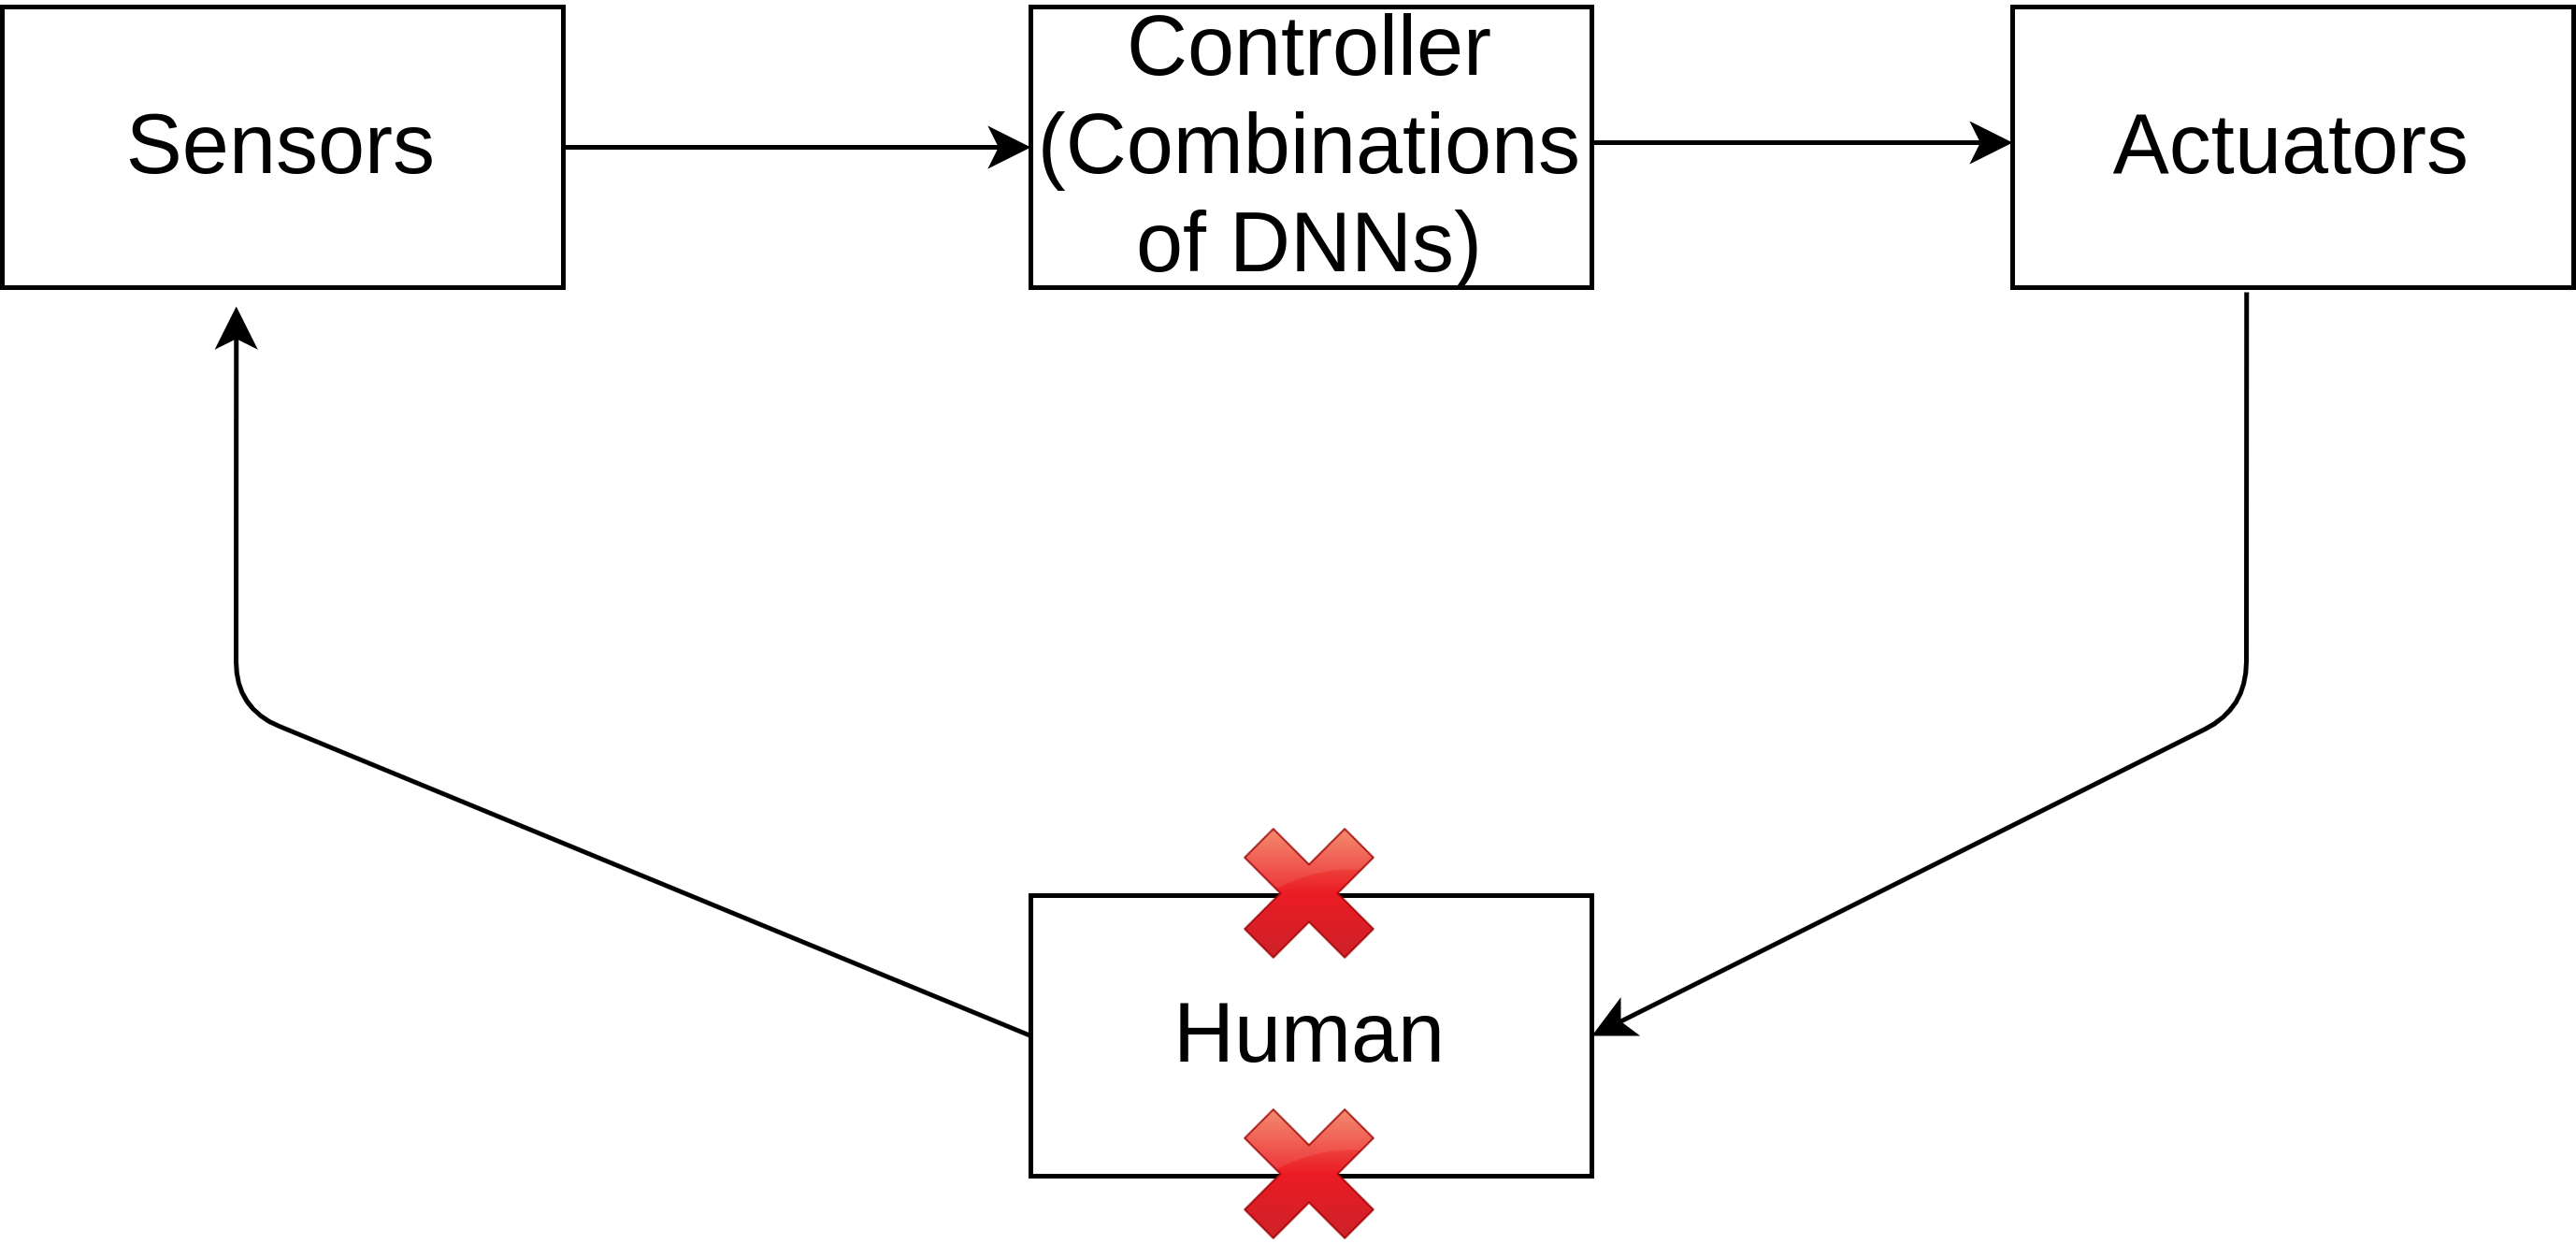
\includegraphics[width=0.7\linewidth]{Images/Systemsdescription}
	\caption{Architecture of a CPS}
	\label{fig:systemsdescription}
\end{figure}

\begin{figure}
	\centering
	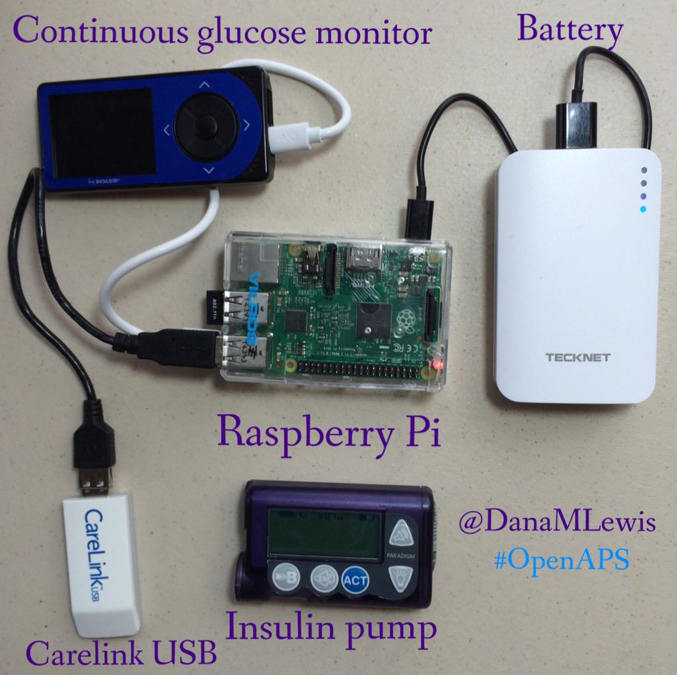
\includegraphics[width=0.7\linewidth]{Images/APSrig}
	\caption{Artifical Pancreas System components \\
		Source: www.openAPS.org}
	\label{fig:apsrig}
\end{figure}



\begin{figure}
	\centering
	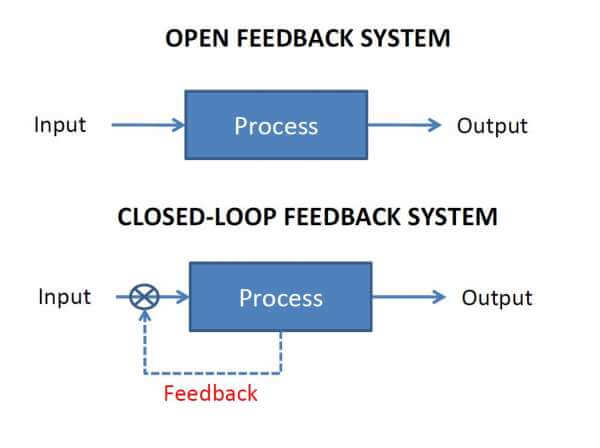
\includegraphics[width=0.7\linewidth]{Images/closedvsopen}
	\caption{General structure of a open and closed-loop systems 
		Source:https://instrumentationtools.com/open-loop-and-closed-loop-animation/ }
	\label{fig:closedvsopen}
\end{figure}


\section{Cyber-Physical Systems}
\ac{CPS} are systems that perform computations in the cyber part to reflect changes in the physical  part.   
As shown in Figure ~\ref{fig:systemsdescription} the sensors and actuators are the physical parts of the system. 
The sensors gather the data from the physical environment and send it to the computational unit. 
The decision is taken at the computational unit which is also the cyber part of the \ac{CPS} called the controller.
The decision is sent to the actuator which then physically performs the action.
The physical and virtual contexts can either be humans in the loop or some automated mechanism.

In an \ac{APS} shown in Figure ~\ref{fig:apsrig}, the sensor is the \ac{CGM} that is attached to the back of a patient to report the blood glucose levels.  
\ac{RPi} is the computational part of the \ac{APS}, and the insulin pump is the actuator. 

There are two types of CPS based on the decision making process: open feedback and closed-loop feedback.
In open feedback systems, 
%there is human intervention during the decision making process. 
as shown in Figure ~\ref{fig:closedvsopen} (top diagram), the human is a part of the loop where he/she keeps track of the decisions being taken by the controller. 
In closed-loop systems, there is no human intervention 
as shown in Figure ~\ref{fig:closedvsopen} (below diagram). 
In the latter case, understanding different types of security attacks becomes a necessity because the automation means that once the attacker has found a way to tamper with the automation mechanism, they can fool the system. 
In the case of stealthy (or subtle) attacks as described in Chapter 3, \karthik{Symbolic ref} 
the closed loop systems are more vulnerable because existing error-detection mechanisms can be reverse engineered and can be used to attack the systems. 

\section{Conventional Controllers for CPS}

A conventional controller takes in the sensors readings and processes the input based on the different sets of differential equations for the controller. 
For instance, a quadcopter contains multiple flight modes in its controller based on the weather conditions such as windy or normal day. 
These modes are important because during windy weather, the decision making model for stable quadcopter flights will be different from a normal weather flight \cite{inbook}. 

Based on the inputs or data collected from the sensors, the appropriate  mode is selected and the decision is calculated. 
Every mode consists of a different set of equations because every mode represents a different scenario.
Figure ~\ref{fig:controltheory} shows a position control system of a quadcopter \cite{inbook}. The input values use the derived version of the equations that are used in decision making. 

\begin{figure}
	\centering
	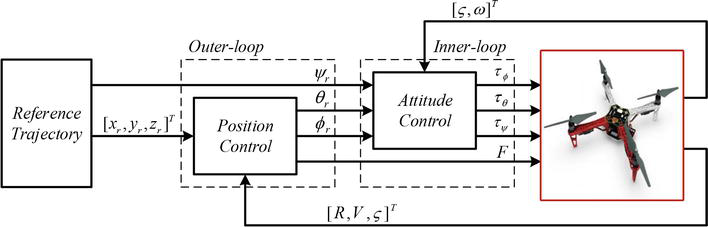
\includegraphics[width=0.7\linewidth]{Images/controltheory}
	\caption{The block diagram of the position control system of the quadcopter.
	}
	\label{fig:controltheory} 
\end{figure}


%How are they modeled
These modes are modeled using classical control theory that is represented as a set of equations designed by domain experts.
For instance, the model for a medical system such as \ac{APS} can be designed only if the specifications are known for the medical system. 
A part of the specifications such as the important parameters (insulin, blood glucose etc. in APS) and their threshold values are be provided by domain (in this case medical) experts. 
Another important aspect for designing control systems is modeling the precise relations between the parameters. 
This is possible in systems such as APS because it is a simpler system as compared to self-driving cars. 
However, designing the precise mathematical relations for systems such as self-driving cars can be tedious \cite{article23}, as we elaborate below.

The move towards DNNs over control theory models for modeling \ac{CPS} behaviour can be justified by the following observations:
\begin{enumerate}
	\item CPS behaviour is controlled using a lot of input data from the many sensors a system might have. The self-learning nature of DNNs lends itself well to model behaviour that is driven by the sensor input. This is easier than formulating the control theoretic differential equations, which need domain and mathematical expertise \cite{Aamir_2013}.
	
	
	To look at a more concrete example, let us turn to a medical system such as \ac{APS}, which uses conventional control theory to build models. 
	Forming the model requires the programmer to be aware of not only the intended system behaviour, but also the mathematical rigor needed to get the desired result. 
	DNNs, on the other hand, can automatically build models with data.
	Training DNNs is implicitly dependent on the quality of available training data, and it is a known problem in the field \cite{jabbar2015methods}. It does not, however, require the system designers to model precise control equations like in control theory.
	\item  There are limitations on the behaviors that can be modeled using the standard control-theoretic approaches. They do not, for instance, work well for building dynamic models \cite{article23}. Building such dynamic models is important in many systems such as in autonomous vehicles, which are essentially composed of multiple interacting control systems. Conventional control systems are not designed to work in an interactive, plug-and-play manner with other control systems because they are built to model only one behaviour. DNNs, by their very nature,  provide this dynamic capability \cite{article23}. 
	Due to the data driven modeling using DNNs, it is relatively easier to build models for autonomous vehicles that have multiple models interacting within them.
	For instance, they contain separate models for image recognition and lane detection that continuously interact with each other to decide the next best course of action.
	
	\item Sarabakha et al. \cite{sarabakha2019online} show that using \ac{DNN} based controller for a quadcopter leads to better decision making in unspecified cases as compared to control theory models.
	This is due to the learning nature of \ac{DNN}s in contrast to the fixed nature of conventional control theory. 
	Hence, in cases when the trajectories or situations are not precisely modeled, the \ac{DNN} comes closer to taking good decisions.
\end{enumerate}




\section{DNN Based Controller}
\label{apsdnn}


%A \ac{NN} is an algorithm that is modeled after the human brain.
A \ac{NN} consists of input, output and hidden layers. 
The layers are built of nodes. Every computation occurs within in a node of a network.
In the base case, there is a single neuron that takes all the inputs to produce an output as shown in Figure 2.5. 
All inputs to the node in Figure 2.5 are summed up, and  passed through an activation function. 
The activation function introduces non-linearity in the network. 
The node determines up to what extent the signal must be progressed \karthik{seems awkward} to calculate the final output. 
The final output depends on the network and can be in binary form or have a value associated with it. 


A \ac{DNN} consists of multiple hidden layers as apposed to our base case  as shown in Figure 2.7.
This is an example of a feed-forward \ac{DNN} which is the simplest type of artificial neural network devised \cite{feedforward}.
In this network, the information flows only forward from inputs, through layers, to outputs \cite{Zell}. 

The classical controller model is being replaced by such DNN based controllers for CPS as shown in  Figure 2.6.
The \ac{DNN} for \ac*{CPS} is trained using the data gathered from conventional control equations. 
One example is the DNN based controller designed by Dutta et al. \cite{Dutta_Others__2018__Robust}. 
Dutta et al. model robust DNN using available patient data to predict the output for an insulin pump.
Their controller design is for providing a data-driven approach for an artificial pancreas system (APS), which is also our first system for evaluation. 

We evaluate two other systems called \ac{CA} systems for unmanned vehicles \cite{7778055} called \ac{HCAS} and \ac{ACAS-Xu}: both \ac{CA} systems are bigger in size (number of nodes and layers) and have a complex architecture in terms of design as compared to \ac{APS}.


%Normalization layers in DNN
\ac{DNN}s also consist of a feature called normalization in their layers. 
This feature exist mostly in \ac{DNN}s as compared to other \ac{ML} models such as decision trees, since \ac{DNN}s involve less feature engineering as compared to other models. 
Feature engineering is an automatic method to extract features from raw data. 
Normalization is a common feature engineering method where all the inputs are brought to standard scale since different set of inputs can be in different ranges. 
This is important in \ac{DNN}s for reasons explained by  LeCun et al.  \cite{10.5555/645754.668382}.
%The first reason is trivial as computations on a bounded range of numbers prevent some numerical inaccuracies and limit the computational power required. The second reason is that some machine learning algorithms can handle that data better when it is normalized. There are several approaches to normalization of the data.
Our other two evaluation systems are aircraft  control management systems \cite{10.1007/978-3-319-63387-9_5} that consist of a normalization layer, 
which we have to consider in our system modeling. 
\subsection{Understanding DNN complexity}
\label{dnncomplexity}
To understand the complexity of \ac{DNN}s we use two criteria
\begin{enumerate}
	\item Size: The size depends on two aspects, the number of layers in a \ac{DNN} and the number of nodes in each layer. 
    The increase in the hidden layers corresponds to more connections and opacity between the inputs and the outputs. 
    The increase in the number of nodes per layer corresponds to more connections between each layer which ultimately increases the opacity of the input and output mapping. 
	\item Architecture: The architecture consists of the the design of the network. 
	For a fully-connected network, every node is connected to every other node in the network, and it contains ReLU or some other activation function to introduce non-linearity.
	Other networks also consist of layers that perform max/average pooling operations. 
	
\end{enumerate}
When we refer to \ac{DNN} complexity in this thesis, we are referring to the differences in size and architecture.


\begin{figure}
	\centering
	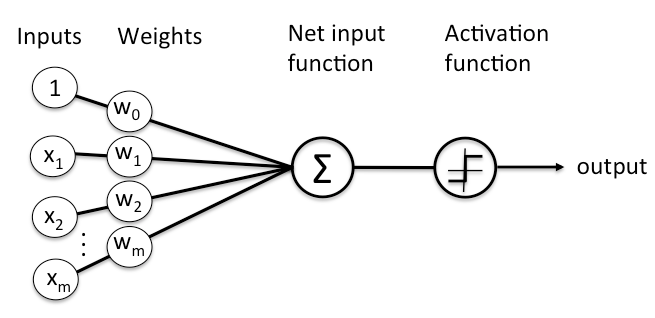
\includegraphics[width=0.7\linewidth]{Images/perceptron_node}
	\caption{Perceptron node  \\ Source: https://pathmind.com/wiki/neural-network}
	\label{fig:perceptronnode}
\end{figure}

\begin{figure}
	\centering
	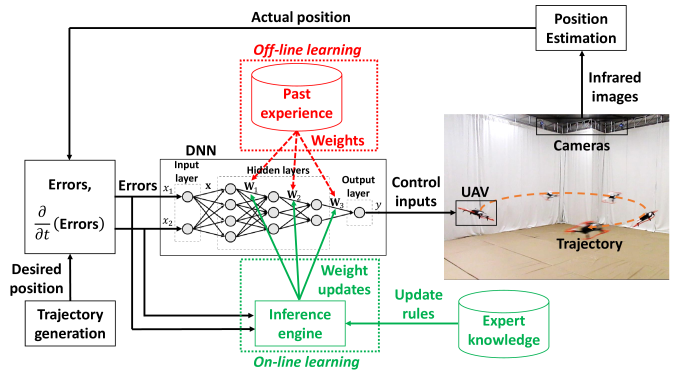
\includegraphics[width=0.7\linewidth]{Images/DNNcontroller}
	\caption{Illustration of how DNN controllers are replacing conventional controllers. The DNN is trained offline using input-output data obtained from different trajectories from a conventional controller. The DNN is shown to perform better than a conventional controller during real-time analysis for decision making.}
	\label{fig:dnncontroller}
\end{figure}

\begin{figure}
	\centering
	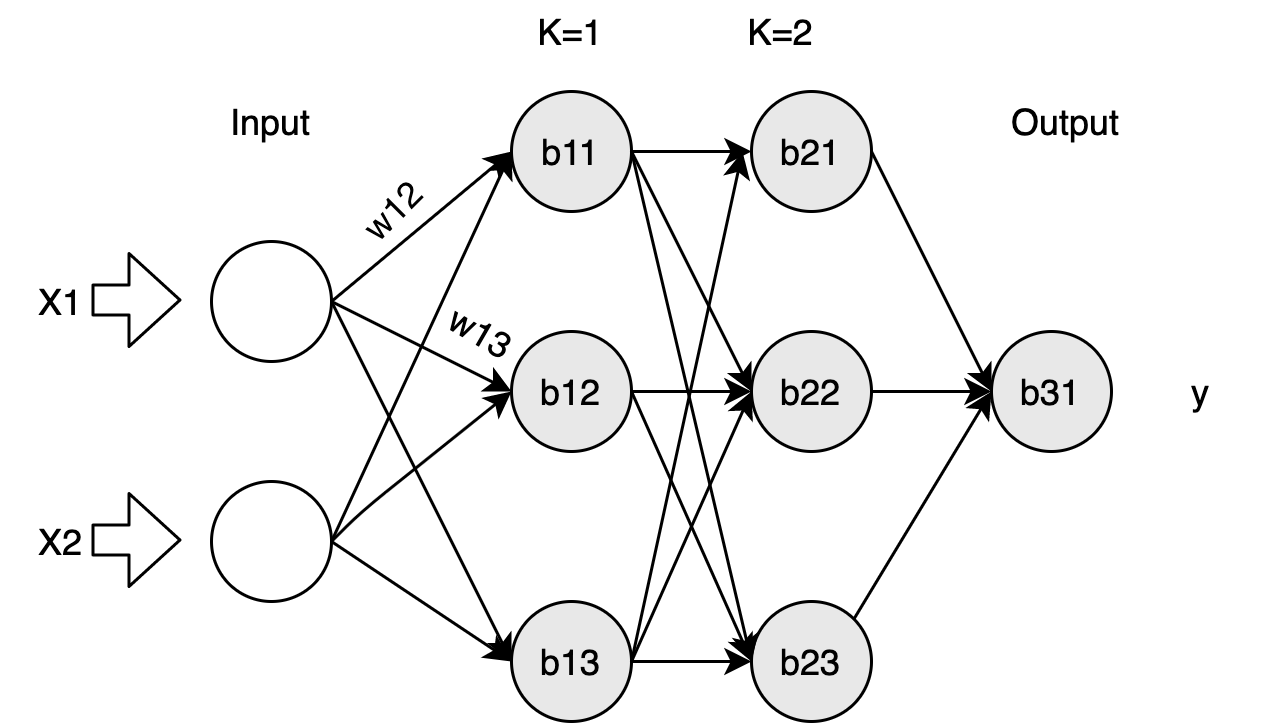
\includegraphics[width=0.7\linewidth]{Images/DNNstructure}
	\caption[DNN structure]{DNN controller structure with two hidden layers K=1,2, two inputs x1 and x2 and one output y. This is an example of a fully connected network.}
	\label{fig:dnn-controller}
\end{figure}

\section{Modeling Mixed-Integer Linear Programming Problems}
\label{milp}
We present a general structure that is required for building a \ac{LP} \ac{MILP} models.
The reason we are introducing the notion of \ac{MILP} is because we use the modeling techniques underlying \ac{MILP} to model \ac{DNN}s and systematically reason about them. 
An \ac{LP} is characterized by the following components. 

\begin{enumerate}
	\item A \ac{LP} contains a set of decision variables, which are the unknown quantities or decisions that are to be optimized. 
	\item The function that assess the quality of the solution is called an objective function or the cost function.
	\item \ac{LP}'s goal is to minimize or maximize the value of an objective function. 
	The decisions that are to be made depends on the requirements, and restrictions of the  system modeled as \ac{LP}.
	\item A solution that satisfies all constraints is called a feasible solution. 
	Feasible solutions that achieve the the best cost function value, depending on weather one is minimizing or maximizing are called as optimal solutions. 
\end{enumerate}


The general form of a \ac{LP} looks as shown in Equations 2.1. 
Values of $c$ denote the objective coefficients, and are often associated with their corresponding decisions minimization problems. 
$x_i$ denotes the set of our decision variables.
$b_i$ denotes the requirements of the constraints. 
A very important point here is that nonlinear terms are not allowed in the model. 
Hence, something as simple as multiplication of two decision variables is prohibited in the model representation. 
\begin{equation}
\begin{aligned}
& \underset{x}{\text{min/max}}
& & c^T x \\
& \text{subject to} & &  Ax \leq b_i \\
& & &  \sum_{i=1}^{n} x_i =1 \\
& & &  x_j, \; \forall j \in N. \\
\end{aligned}
\end{equation}

A \ac{MILP} is a \ac{LP} with a restriction that some of the variables in the model must be integer-valued. 
We define a \ac{DNN} as a \ac{MILP} model due to the complex structure of a \ac{DNN} which we will elaborate more in Chapter ~\ref{evaluation}. 

There are multiple tools that provide an interface to build \ac{MILP} models such as Cplex ~\cite{cplex}, and Gurobi ~\cite{gurobi}.
Both are high-performing tools\karthik{What's a high-performing tool?}; however, we choose Gurobi for our purpose as it was more usable\karthik{Please check}. 



\section{Problem Statement}
\label{problemstatement}

Given a trained DNN with fixed parameters our goal is to understand if the well-known \ac*{FDIA} in classical control theory are also valid in the DNN based CPS. \karthik{Given that we've introduced RFDIA, should we simply say RFDIA here?} \karthik{and to automatically mount them, correct ?}
This leads to two sub-problems as follows.

\begin{problem}
	How can we identify the critical inputs in a DNN?
\end{problem}

\begin{problem}
	What is the smallest perturbation to the critical input(s) that can produce \ac{RFDIA}?
\end{problem}





%    2. Main body
% Generally recommended to put each chapter into a separate file
%\chapter{Related Work}
\label{ch:Chapter2}



We have classified related work into four broad categories. The first category discusses the verification techniques that have emerged to verify DNNs. We highlight why those techniques cannot directly be used for our application. The second discusses work done in the FDIA community for classic control theory modeled systems and why our work is required to understand the consequences of deploying DNNs in CPS.  In the third category, we discuss multiple applications where DNNs have replaced the traditional CPS. This provides a glimpse into how the DNNs are being utilized in safety-critical applications. Furthermore, this motivates the need for a technique that can generalize to different settings of DNN based CPS. Finally, in the last category we discuss the adversarial attacks that have gained a lot of attention in the Machine Learning community and how are they different from our \attack. 
\subsection{Verification of CPS}
%Providing formal guarantees for CPS has always been an important part of the literature. The reason is due to their safety-critical nature. 

%\subsection{Control Theory CPS }
%\subsection{DNN based CPS}
Formally verifying DNN based CPS has recently gained a lot of momentum. Researchers have proposed automated verification mechanisms that use techniques involving SMT solvers, symbolic execution and MILP. However, the modeling that has been done for those interfaces cannot be directly used for our use case without modifications. The goal of these techniques is to conduct an input-output range analysis to establish bounds for the DNN. Our work focuses not on conducting a bound analysis but finding the optimal inputs for changing the outcome of a CPS under a constrained setting for a FDIA. Also, the approaches focus more on verifying certain properties such as reachability analysis that do not account for \attack.

Pulina et al.\cite{10.1007/978-3-642-14295-6_24} proposed one of the first approaches for verifying DNN safety properties using abstraction refinement. They further abstract \cite{article} the nonlinear activation functions in a linear arithmetic SMT formula. They then use counterexample based approach for abstract refinement. There has been further work by Katz et al.\cite{10.1007/978-3-319-63387-9_5} in verifying the networks using SMT solvers where they build rules for handling the ReLU activation function. Most of work we have mentioned above in this domain utilizes the state-of-the art solvers Z3 and CVC4. However, all the existing techniques focus on proving robustness properties \cite{NIPS2016_6339} for DNNs that cannot detect or produce FDIA. Xiang at al.\cite{xiang2017output} focuses on an output reachable estimation for NN using simulation-based methods. There have been multiple methods proposed to conduct a rechability analysis for DNN using MILP/SMT approach \cite{10.1145/3302504.3313351} \cite{ehlers2017formal} \cite{10.1007/978-3-319-63387-9_5} \cite{lomuscio2017approach} \cite{article}. Ivanov et al. \cite{ivanov2018verisig} proposes a verification framework for verifying DNN based controllers by abstracting the problem into a hybrid system verification problem.  
%\subsection*{Cyber-Physical Systems Security}
%Sensor spoofing attacks- multiple types such as gps spoofing, most common ones demonstrated are FDI.

\subsection{False Data Injection Attacks (FDIA) in traditional systems}
%FDI attacks in CPS in different domains. Difference in terms of modelling of systems. Sparse FDI attacks
Attacking the CPS by exploiting the deep integration of the physical-nature and cyber nature of the systems has lead to the emergence of FDIAs. 
There are two main categories of FDI attacks that have been proposed in the literature: random FDIA and targeted FDIA. Random FDIA are generated by randomly changing the inputs to cause changes in the state estimation. Targeted FDIAs are the more interesting ones from an attackers perspective because in this case, they have to synthesize the exact values of inputs to cause a change in the output without triggering alarms. Our work focuses on synthesizing random and targeted FDIAs under specific set of constraints based on the specification documentation. 

In FDI attacks, the attacker's goal is to compromise the sensor inputs to mislead the state estimation process \cite{e3f0020abba24d4389aff937fe8bcdd5}. Liu et al. \cite{10.1145/1952982.1952995} introduced the class of FDIA for electric power grids to introduce arbitrary errors into certain state variables without being detected. Giannini et al. \cite{unknown} generate FDIA under specific setting %\karthik{What does this mean?}
where they introduce new information as constraints in the state estimator under the assumption that the new information is not available to the attacker. This can basically be seen as security by obscurity. These techniques generate FDIA for systems modeled using control theory in order to cause a wrong state estimation without getting detected. Our work looks at the CPS constructed using \ac{DNN}. We try to understand if \ac{FDIA} would work in different constraint setting. Bobba et al. \cite{Bobba2010DetectingFD} show that by protecting a strategically selected set of sensor measurements it is possible to detect the attacks proposed by Liu at al. \cite{10.1145/1952982.1952995}.
% Bai et al. \cite{bai2020aigan} proposes AI-GAN which provides a boost up over previous adversarial examples techniques. In contrast, our work is not focusing on adversarial examples for DNNs but FDIA for DNN based CPS in a constrained environment. 

\subsection{DNN controllers in CPS}
This section focuses on intelligent control primarily due to the introduction of neural networks(NN) in designing the control systems. This subsection discusses how different types of \ac{DNN} are utilized in \ac{CPS} modeling. There are multiple types of \ac{DNN} architectures that have been proposed by \ac{CPS} designers in the recent years. This work is mentioned to provide an intuition of the different models that exist and how none of them have a common means of abstraction or representation.   %As discussed in the Problem Formulation section NN allow the input-output mapping because of the nodes connecting in a network.


Fukuda et al. \cite{170966} show how NN can be utilized in multiple industrial systems. Cong et al. \cite{Cong} proposes a recurrent neural network that is used to create a PID neural network (PIDNN). A proportional–integral–derivative controller is a control loop mechanism employing feedback that is widely used in industrial control systems and a variety of other applications requiring continuously modulated control. This allows the network to converge faster since PIDNN has one hidden layer with 3 neurons that represent K$_p$, K$_i$ and K$_d$ that are used in traditional PID controllers. Wang et al. \cite{Wang2016ACA} proposes a double layer architecture for a non-linear system using adaptive NN control and Nonlinear Model Predictive Control (NMPC). However, none of the mentioned work explores the security affects of replacing the standard controllers with DNNs. Our work specifically looks into understanding the affects of replacing the standard controllers with DNNs and \attack is one of the results.

\subsection{Deep Neural Network Security}
%ML security such as adversarial ML
%adding noise to the inputs to change classification but they are based on RNN and other such networks- we use MILP optimization in order to find attacks that cause slight deviations and do not necessarily change the output
%DNNs are susceptible to attacks as is.

The deep learning security comprises the adversarial examples field which was introduced by Szegedy et al. \cite{Szegedy2013IntriguingPO} where they showed that the input-output mappings for the DNNs are not continuous and it is possible to perturb the inputs by small amounts such that the classification changes. Since then there has been a lot of work exploring different types of adversarial attacks. There are two ways of attacking the \ac{ML} models: data poisoning \cite{DBLP:journals/corr/abs-1903-01666}, and adversarial attacks broadly survey by Papernot et al. \cite{DBLP:journals/corr/PapernotMSW16}. Data poisoning attacks perturb the data during the training phase of the networks whereas adversarial attacks usually act on a trained network by falling the specific input set that creates erroneous perturbations in the output. 



 Deng et al. \cite{deng2020analysis} analyses five types of adversarial attacks in autonomous driving models.  ConAML \cite{li2020conaml} explores the constrained adversarial attacks for cyber-physical systems under different settings. They propose a best effort algorithm to iteratively generate adversarial examples. We on the other hand introduce \attack  that generate ripples based on constraints. We are not trying to find inputs that cause erroneous perturbations due to the deviations but due to the design of the systems. 
  Wang et al. \cite{217595} proposes ReLUVal that uses symbolic execution to show that the DNN based systems are free from security vulnerabilities. They use symbolic execution to ensure that in specific intervals the system is free from attacks whereas we formalize the \ac{CPS} using \ac{MILP} . 

%The goal of our work is to find if a DNN based CPS has ripples and to do so we use MILP whose goal is to find a \attack if it exists.
% \karthik{What about the ReLuVal paper [37] ?}

%\aarti{Add more papers here}
%CPS verification 
%\include{model}
%\include{impl}
%\chapter{Discussion}
In this section we discuss how to model our insights into modeling robhust \karthik{Spell Check Fail!} 
DNNs by two approaches. \karthik{Did you mean leverage insights ? Also, what're the approaches for ?} 
We also discuss some limitations in our approach.

\section{Designing Robust DNNs}
From our experience in working with three different types of DNN based CPS to attack the systems, we realized that there are two ways to construct or build robust DNN based systems. 
\karthik{Can you say a little bit about how you came to this realization ? Was it based on the experimental results ?}

\section{Designing Robust DNN from scratch}
The biggest difference between APS and ACAS Xu apart from the DNN size was the robustness of the DNN. APS had a simple feed-forward architecture, where the network took the inputs, applied the non-linearity to the equations \karthik{non-linearity is not an action !},
 and calculated the outputs. Whereas ACAS Xu applied normalization to its inputs. \karthik{This is a phrase, not a sentence}

APS had accompanying DNNs that kept\karthik{Duh ?} did a range check to ensure that the output prediction lies within certain bounds \karthik{Did you mean specified bounds ?}. 
This was easier to break as per our attack model as compared to ACAS Xu\karthik{Can we quantify easier? Also, by break, I guess you mean attack?}. 
In ACAS Xu, due to the normalization of the inputs, the perturbations had to be carefully designed since one input perturbation did not easily perturb the outputs easily \karthik{Too many easilys!}. 
We can also observe the percentage of successful attacks from Table II \karthik{Symbolic ref.?} in APS and ACAS Xu. \karthik{What did you observed about them?}
Hence, we believe that applying techniques while training and modeling DNN architecture can significantly help prevent \attack. \karthik{This is a vacuous statement. What techniques are these ? How does one go about designing such a DNN?}

\section{Debugging existing DNN using \tool}
Given there exists a system with DNN similar to that of APS without inbuilt mechanisms, we believe that our tool can help in debugging the DNN by constructing a comprehensive list of cost functions and running the model for different scenarios. This might not provide complete coverage but can certainly help in the falsification process. 
\karthik{So what's falsification here. Also, it seems like an overly restrictive statement to make about the similarity with APR. What's inbuilt mechanism here ?}

\section{ Limitations}

There are 2 limitations in our work.
First, we are assuming that the attacker has access\karthik{Read or write ? Be specific !} to the weights and the bias. However, in a more ideal attack scenario \karthik{for the attacker ?}, if we \karthik{Who's we?} can find a way to  attack the system without knowing the weights and bias of the system, that would be really interesting \karthik{Please avoid weasel words like interesting - make it clear what is of interest}. %Figuring out FDI attacks in that scenario would be challenging yet rewarding. 
Second, for bigger systems such as ACAS Xu, we observed that running all combinations was taking a lot of time (approx 13 hours), only to tell us that no attack exists \karthik{I suppose us is we as the researcher here. Also, is the time taken a function of the attacks or the network ?}. We think there is scope of improvement to provide speedups by applying clever heuristics to the model. \karthik{Perhaps give 1-2 examples of heuristics here.}


%The limitation of our work is that we do not evaluate the completeness of our approach. We show experimentally that our technique always provides us a solution if the model is properly modeled and if there are attacks possible. Otherwise, it returns an infeasible model.  Since the modeling of the network is represented as a set of well-defined equations it is always going to return a solution if it exists. If no solution exists then it will return the model is infeasible. 
%The interesting part of our approach is that we are not trying to verify but instead we are trying to find feasible FDI attacks for the system. 
\label{section:limitations}
%\include{conclusions}

%    3. Notes
%    4. Footnotes

%    5. Bibliography
\begin{singlespace}
\raggedright
	\bibliography{bib}
\bibliographystyle{ieeetr}
\end{singlespace}

\appendix
%    6. Appendices (including copies of all required UBC Research
%       Ethics Board's Certificates of Approval)
%\include{reb-coa}	% pdfpages is useful here

%\include{appendix}

\backmatter
%    7. Index
% See the makeindex package: the following page provides a quick overview
% <http://www.image.ufl.edu/help/latex/latex_indexes.shtml>


\end{document}
